% Chapte 7
\chapter{Advertisement application} % Main chapter title

\label{Chapter7} % For referencing the chapter elsewhere, use \ref{Chapter1} 

\section{Introduction}
The use of technology in advertisement plays a major role in advertisement industries, it would have been much difficult to reach to their customers without technologies, and technology enhances the two-way communication much with client and customers. The companies can now easily express their thoughts and vision to their customers with the use new technologies. Advertisement are everywhere like in websites, in your smartphone, in Television and radio and especially from past decade it is more common on the streets, supermarkets, airports and areas where is crowded, So for every context or setting there are set of technologies that are being used to make the advertisement more appropriate, and when it comes to interactive advertisement the use of right technology plays another major role in terms of usability and understandability, Interactive advertisement in websites are usually interactive using keyboard and mouse, in smartphone is using the capability of the touch or other sensors to make the interaction easy and at the same time funny, and interactive advertisement in public space has again another bunch of technologies that could make the interaction usable like using face recognition, body and position recognition, hand gesture recognition and also touch sensors, proximity sensors and much more.

This chapter explains all the technical aspects of advertisement system that were developed during the thesis work. This chapter discusses what technologies and hardware have been used and what algorithm and methods have been implemented to accomplish the goals. This chapter explains the software for three main parts, attracting attention application, main advertisement application and the enhanced advertisement application.


\section{Attracting attention Application}
The goal of attraction attention was to develop systems that could attract the attention of the passers-by, in which three different applications were developed and later compared.

\subsection{Requirement gathering}
The bellow are the required elements used for the applications.


\subsubsection{Hardware requirement}

\begin{itemize}
\item \textbf{Microsoft Kinect Camera} \cite{Kinect} \\
This is one of the most used camera in public context a lot, this camera can track up to seven user's position (X, Y, Z) in real time; it is capable of recognizing hand gesture and even can track facial movements. The camera does not work well when it is exposed in sunlight, which makes it ideal for indoor use only. In our experiment Microsoft Xbox 360 Kinect camera was used, The Kinect camera should be used with an extra adapter in order to connect it to computer. 
\item \textbf{Computer} \\
A normal laptop was used with Core i7 2.7 Ghz processor, and 4 GB RAM and USB of 2.0 version.
If you want to use Xbox Kinect One Kinect then the computer should support USB version 3.0.
The laptop was connected to the University monitor via mini display port.

\end{itemize}


\subsubsection{Software requirement}
The software can run in any operating system except because of the processing programming language. In experiment mac OSX operating system was used with bellow library and processing version.
\begin{itemize}
\item Processing v2.2.2 or higher version.
\item SimpleOpenNI library for Processing \cite{simpleopenni}
\item 32bit JRE (Java Runtime Environment) v1.8 or higher.
\end{itemize}


\subsection{Following eye application}
The name is given \emph{Following eye} because the application shows eyes for each individual when pass from the front of the screen and those eyes follow the person where they walk. The interaction works with the Kinect camera that provides each individual positions.
Explore the attached CD for the source code.

\subsection{Firework application}
This application also uses kinect camera to track user position and renders a firework animation for each person.
The fireworks are created with using random number of circls (balls) with random colors and sizes, the circles burst from the person's location and spreads to random directions with a high speed and slows down at the end. One part of the application's code is freely taken from openprocessing community that could generate random firework bubbles.
For more detail please check the CD for source code.

\subsection{Silhouette application}
This application uses Kinect camera to produce colored silhouette of passers-by, the camera has a resolution of 640x480 pixels and the application requests UserMap from Kinect camera, userMap is a 1xD integer array from that corresponds to the pixels of the Kinect image, which normally looks like bellow. \\

\emph {Int upix = context.userMap();}

\emph{upix = [1,1,1,1,1,1,1,2,2,2,2,2,2,2,2,2,-1,-1,-1,-1,-1,-1,2,2,2,2,....]}

The above example shows the structure of the array, the index of the elements of array correspond to the pixel number of image and the element values correspond to the user id standing in front of the camera, the user id is always above zero, any value which is not above zero in fact could be background or non-user pixel, the example shows that there are at least two people standing in front of the camera, which has user id (1 and 2) the -1 value is a non-user pixels. 
So the application iterates to this array and assigns specific color to each of the pixels of the user image and does not give color to the non-user pixels. 


% Please add the following required packages to your document preamble:
% \usepackage[table,xcdraw]{xcolor}
% If you use beamer only pass "xcolor=table" option, i.e. \documentclass[xcolor=table]{beamer}
% Please add the following required packages to your document preamble:
% \usepackage[table,xcdraw]{xcolor}
% If you use beamer only pass "xcolor=table" option, i.e. \documentclass[xcolor=table]{beamer}
% Please add the following required packages to your document preamble:
% \usepackage[table,xcdraw]{xcolor}
% If you use beamer only pass "xcolor=table" option, i.e. \documentclass[xcolor=table]{beamer}
\begin{table}[H]
\centering
\caption{UserMap and application color mapping}
\label{usermap_colormapping}
\resizebox{\textwidth}{!}{ 
\begin{tabular}{ccccccccccccccccccccccccccccccccccccccccc}
-1 & -1 & -1                        & -1                        &                           &                           &                           &                           &                           &                           &                           &                           &                           &                           &                           &                           &                           &                           &                           &                           &                           &                           &                           &    &    &    &                           &                           &                           &                           &                           &                           &                           &                           &                           &                           &                           &                           &  &  &  \\
-1 & -1 & -1                        &                           & -1                        &                           & -1                        & -1                        & -1                        &                           & -1                        & -1                        & -1                        & -1                        & -1                        & -1                        & -1                        & -1                        & -1                        & -1                        &                           &                           &                           &    &    &    &                           &                           & -1                        &                           & -1                        &                           & -1                        & -1                        &                           &                           &                           &                           &  &  &  \\
   &    &                           &                           &                           &                           &                           &                           &                           &                           &                           &                           &                           &                           &                           & -1                        &                           &                           &                           &                           &                           &                           &                           & -1 &    &    & -1                        & -1                        & -1                        & -1                        &                           & \cellcolor[HTML]{FE0000}2 & -1                        & -1                        & -1                        &                           &                           &                           &  &  &  \\
-1 & -1 & -1                        & -1                        & -1                        & -1                        & -1                        & -1                        & -1                        & -1                        & -1                        & -1                        & -1                        & -1                        &                           &                           &                           &                           & -1                        &                           &                           &                           &                           &    &    &    & \cellcolor[HTML]{FE0000}2 & -1                        & -1                        &                           & \cellcolor[HTML]{FE0000}2 & \cellcolor[HTML]{FE0000}2 & \cellcolor[HTML]{FE0000}2 & -1                        & -1                        & \cellcolor[HTML]{FE0000}2 &                           &                           &  &  &  \\
-1 & -1 & -1                        & -1                        & -1                        & -1                        & -1                        & -1                        & -1                        & -1                        & -1                        & -1                        & -1                        & -1                        & -1                        & -1                        &                           &                           &                           &                           &                           &                           &                           &    &    &    &                           & \cellcolor[HTML]{FE0000}2 & \cellcolor[HTML]{FE0000}2 & \cellcolor[HTML]{FE0000}2 & \cellcolor[HTML]{FE0000}2 & \cellcolor[HTML]{FE0000}2 & \cellcolor[HTML]{FE0000}2 & \cellcolor[HTML]{FE0000}2 & \cellcolor[HTML]{FE0000}2 &                           &                           & -1                        &  &  &  \\
-1 & -1 & -1                        & -1                        & -1                        & -1                        & -1                        & -1                        & -1                        & -1                        & -1                        & -1                        & -1                        & -1                        & -1                        &                           &                           &                           &                           & -1                        &                           &                           &                           &    &    &    &                           & -1                        & -1                        & -1                        & \cellcolor[HTML]{FE0000}2 & \cellcolor[HTML]{FE0000}2 &                           & -1                        & -1                        & -1                        &                           &                           &  &  &  \\
-1 & -1 & -1                        & -1                        & -1                        & -1                        & -1                        & -1                        &                           &                           & -1                        &                           & -1                        &                           &                           & -1                        &                           &                           &                           &                           & -1                        &                           &                           &    &    &    &                           &                           &                           &                           & \cellcolor[HTML]{FE0000}2 & \cellcolor[HTML]{FE0000}2 &                           &                           &                           & -1                        &                           &                           &  &  &  \\
   &    &                           &                           &                           &                           &                           &                           &                           &                           &                           &                           &                           &                           &                           &                           &                           & -1                        & -1                        &                           &                           &                           &                           &    &    &    &                           &                           &                           & \cellcolor[HTML]{FE0000}  & -1                        & -1                        & \cellcolor[HTML]{FE0000}2 &                           &                           &                           &                           & -1                        &  &  &  \\
   &    &                           &                           &                           &                           &                           &                           &                           &                           &                           &                           &                           &                           &                           &                           &                           & -1                        & -1                        &                           &                           &                           &                           &    &    &    &                           &                           & \cellcolor[HTML]{FE0000}2 & -1                        & -1                        & -1                        & -1                        & \cellcolor[HTML]{FE0000}2 &                           &                           &                           &                           &  &  &  \\
   &    &                           &                           &                           &                           &                           &                           &                           &                           &                           & \cellcolor[HTML]{3531FF}3 & \cellcolor[HTML]{3531FF}3 & \cellcolor[HTML]{3531FF}3 & -1                        &                           &                           & -1                        & -1                        &                           &                           &                           &                           &    &    &    &                           & \cellcolor[HTML]{FE0000}2 & \cellcolor[HTML]{FE0000}2 &                           & -1                        & -1                        &                           &                           & \cellcolor[HTML]{FE0000}2 &                           &                           &                           &  &  &  \\
   &    & \cellcolor[HTML]{3531FF}3 &                           &                           &                           &                           &                           &                           &                           &                           & \cellcolor[HTML]{3531FF}3 & \cellcolor[HTML]{3531FF}3 & \cellcolor[HTML]{3531FF}3 & -1                        &                           & -1                        & -1                        & -1                        &                           &                           & \cellcolor[HTML]{3531FF}3 & \cellcolor[HTML]{3531FF}3 &    &    &    &                           &                           &                           &                           &                           &                           &                           &                           &                           &                           &                           &                           &  &  &  \\
   &    &                           & \cellcolor[HTML]{3531FF}3 & \cellcolor[HTML]{3531FF}3 &                           &                           &                           &                           &                           &                           &                           & \cellcolor[HTML]{3531FF}3 & \cellcolor[HTML]{3531FF}3 & -1                        & -1                        & -1                        &                           &                           & \cellcolor[HTML]{3531FF}3 & \cellcolor[HTML]{3531FF}3 & -1                        &                           & -1 & -1 & -1 &                           &                           &                           & -1                        &                           & -1                        & -1                        &                           & -1                        &                           & -1                        &                           &  &  &  \\
   &    &                           &                           &                           & \cellcolor[HTML]{3531FF}3 & \cellcolor[HTML]{3531FF}3 & \cellcolor[HTML]{3531FF}3 & \cellcolor[HTML]{3531FF}3 & \cellcolor[HTML]{3531FF}3 & \cellcolor[HTML]{3531FF}3 & \cellcolor[HTML]{3531FF}3 & \cellcolor[HTML]{3531FF}3 & \cellcolor[HTML]{3531FF}3 & \cellcolor[HTML]{3531FF}3 & \cellcolor[HTML]{3531FF}3 & \cellcolor[HTML]{3531FF}3 & \cellcolor[HTML]{3531FF}3 & \cellcolor[HTML]{3531FF}3 &                           &                           &                           &                           &    &    &    &                           & -1                        & -1                        & -1                        & -1                        & -1                        & -1                        & -1                        & -1                        & -1                        & -1                        & -1                        &  &  &  \\
   &    & -1                        &                           &                           &                           &                           &                           &                           & \cellcolor[HTML]{3531FF}3 & \cellcolor[HTML]{3531FF}3 & \cellcolor[HTML]{3531FF}3 & \cellcolor[HTML]{3531FF}3 & \cellcolor[HTML]{3531FF}3 & \cellcolor[HTML]{3531FF}3 & \cellcolor[HTML]{3531FF}3 & \cellcolor[HTML]{3531FF}3 &                           &                           &                           &                           &                           & -1                        &    &    &    &                           &                           &                           &                           &                           &                           &                           &                           &                           &                           &                           &                           &  &  &  \\
   &    &                           &                           &                           &                           &                           &                           &                           &                           & \cellcolor[HTML]{3531FF}3 & \cellcolor[HTML]{3531FF}3 & \cellcolor[HTML]{3531FF}3 & \cellcolor[HTML]{3531FF}3 & \cellcolor[HTML]{3531FF}3 & \cellcolor[HTML]{3531FF}3 &                           & -1                        &                           & -1                        &                           &                           & -1                        & -1 & -1 &    & \cellcolor[HTML]{329A9D}1 &                           &                           &                           &                           & \cellcolor[HTML]{329A9D}1 & \cellcolor[HTML]{329A9D}1 &                           &                           &                           &                           & \cellcolor[HTML]{329A9D}1 &  &  &  \\
   & -1 &                           &                           &                           &                           &                           &                           &                           &                           & \cellcolor[HTML]{3531FF}3 & \cellcolor[HTML]{3531FF}3 & \cellcolor[HTML]{3531FF}3 & \cellcolor[HTML]{3531FF}3 & \cellcolor[HTML]{3531FF}3 & \cellcolor[HTML]{3531FF}3 &                           &                           &                           &                           &                           &                           & -1                        &    &    &    & \cellcolor[HTML]{329A9D}1 & \cellcolor[HTML]{329A9D}1 & \cellcolor[HTML]{329A9D}1 & \cellcolor[HTML]{329A9D}1 & \cellcolor[HTML]{329A9D}1 & \cellcolor[HTML]{329A9D}1 & \cellcolor[HTML]{329A9D}1 & \cellcolor[HTML]{329A9D}1 & \cellcolor[HTML]{329A9D}1 & \cellcolor[HTML]{329A9D}1 & \cellcolor[HTML]{329A9D}1 &                           &  &  &  \\
   &    &                           &                           &                           &                           & -1                        &                           &                           &                           & \cellcolor[HTML]{3531FF}3 & -1                        & -1                        & -1                        & \cellcolor[HTML]{3531FF}3 & \cellcolor[HTML]{3531FF}3 &                           &                           &                           &                           &                           &                           & -1                        &    & -1 &    &                           & -1                        &                           & -1                        & \cellcolor[HTML]{329A9D}1 & \cellcolor[HTML]{329A9D}1 & \cellcolor[HTML]{329A9D}1 & \cellcolor[HTML]{329A9D}1 &                           &                           &                           &                           &  &  &  \\
   &    &                           &                           &                           &                           &                           &                           &                           &                           & \cellcolor[HTML]{3531FF}3 & -1                        & -1                        & -1                        & \cellcolor[HTML]{3531FF}3 & \cellcolor[HTML]{3531FF}3 &                           &                           &                           &                           &                           &                           & -1                        &    &    &    &                           &                           &                           &                           & \cellcolor[HTML]{329A9D}1 & \cellcolor[HTML]{329A9D}1 & \cellcolor[HTML]{329A9D}1 & \cellcolor[HTML]{329A9D}1 &                           &                           &                           & -1                        &  &  &  \\
   &    &                           &                           &                           &                           &                           &                           &                           &                           & \cellcolor[HTML]{3531FF}3 & -1                        & -1                        & -1                        & \cellcolor[HTML]{3531FF}3 & \cellcolor[HTML]{3531FF}3 &                           &                           &                           &                           &                           &                           & -1                        &    &    &    & -1                        & -1                        &                           &                           & \cellcolor[HTML]{329A9D}1 & -1                        & -1                        & \cellcolor[HTML]{329A9D}1 &                           &                           &                           &                           &  &  &  \\
   &    &                           &                           &                           &                           &                           &                           & \cellcolor[HTML]{3531FF}3 & \cellcolor[HTML]{3531FF}3 & \cellcolor[HTML]{3531FF}3 & -1                        & -1                        & -1                        & \cellcolor[HTML]{3531FF}3 & \cellcolor[HTML]{3531FF}3 &                           &                           &                           &                           &                           &                           &                           &    &    &    &                           &                           &                           &                           & \cellcolor[HTML]{329A9D}1 & -1                        & -1                        & \cellcolor[HTML]{329A9D}1 &                           &                           &                           &                           &  &  & 
\end{tabular}
}
\end{table}
The above picture has very limited pixels; it is not an original picture but is made to clear the idea of how the coloring of silhouette  works.
As you can see from above picture, the white areas or the -1 values are background and non-user and the remaining positive number represent the pixelse related to the user.
For more information about the source codes, please refer to the CD.


\section{Main advertisement application}
In this section the main advertisement applications are being discussed.
According to the plane there was a need to develop three-advertisement application (non-interactive, body interactive and mobile interactive), which had the same functionality but were different in terms of interactivity and control.

The advertisement application was designed to show important places of Bauhaus that were included in Bauhaus-Walk tour, the pictures of these places are attached on top of the Weimar map with a name on top and a small description at bellow this technique helps participants to build a relationship of location and the map, only five locations are randomly chosen by the software to be shown on the map, each come one after another and when all the locations are explored then the advertisement video will be played and after that the application will repeat it self.

\newpage
\subsection{Interfaces}

\begin{figure}[H]
    \centering
    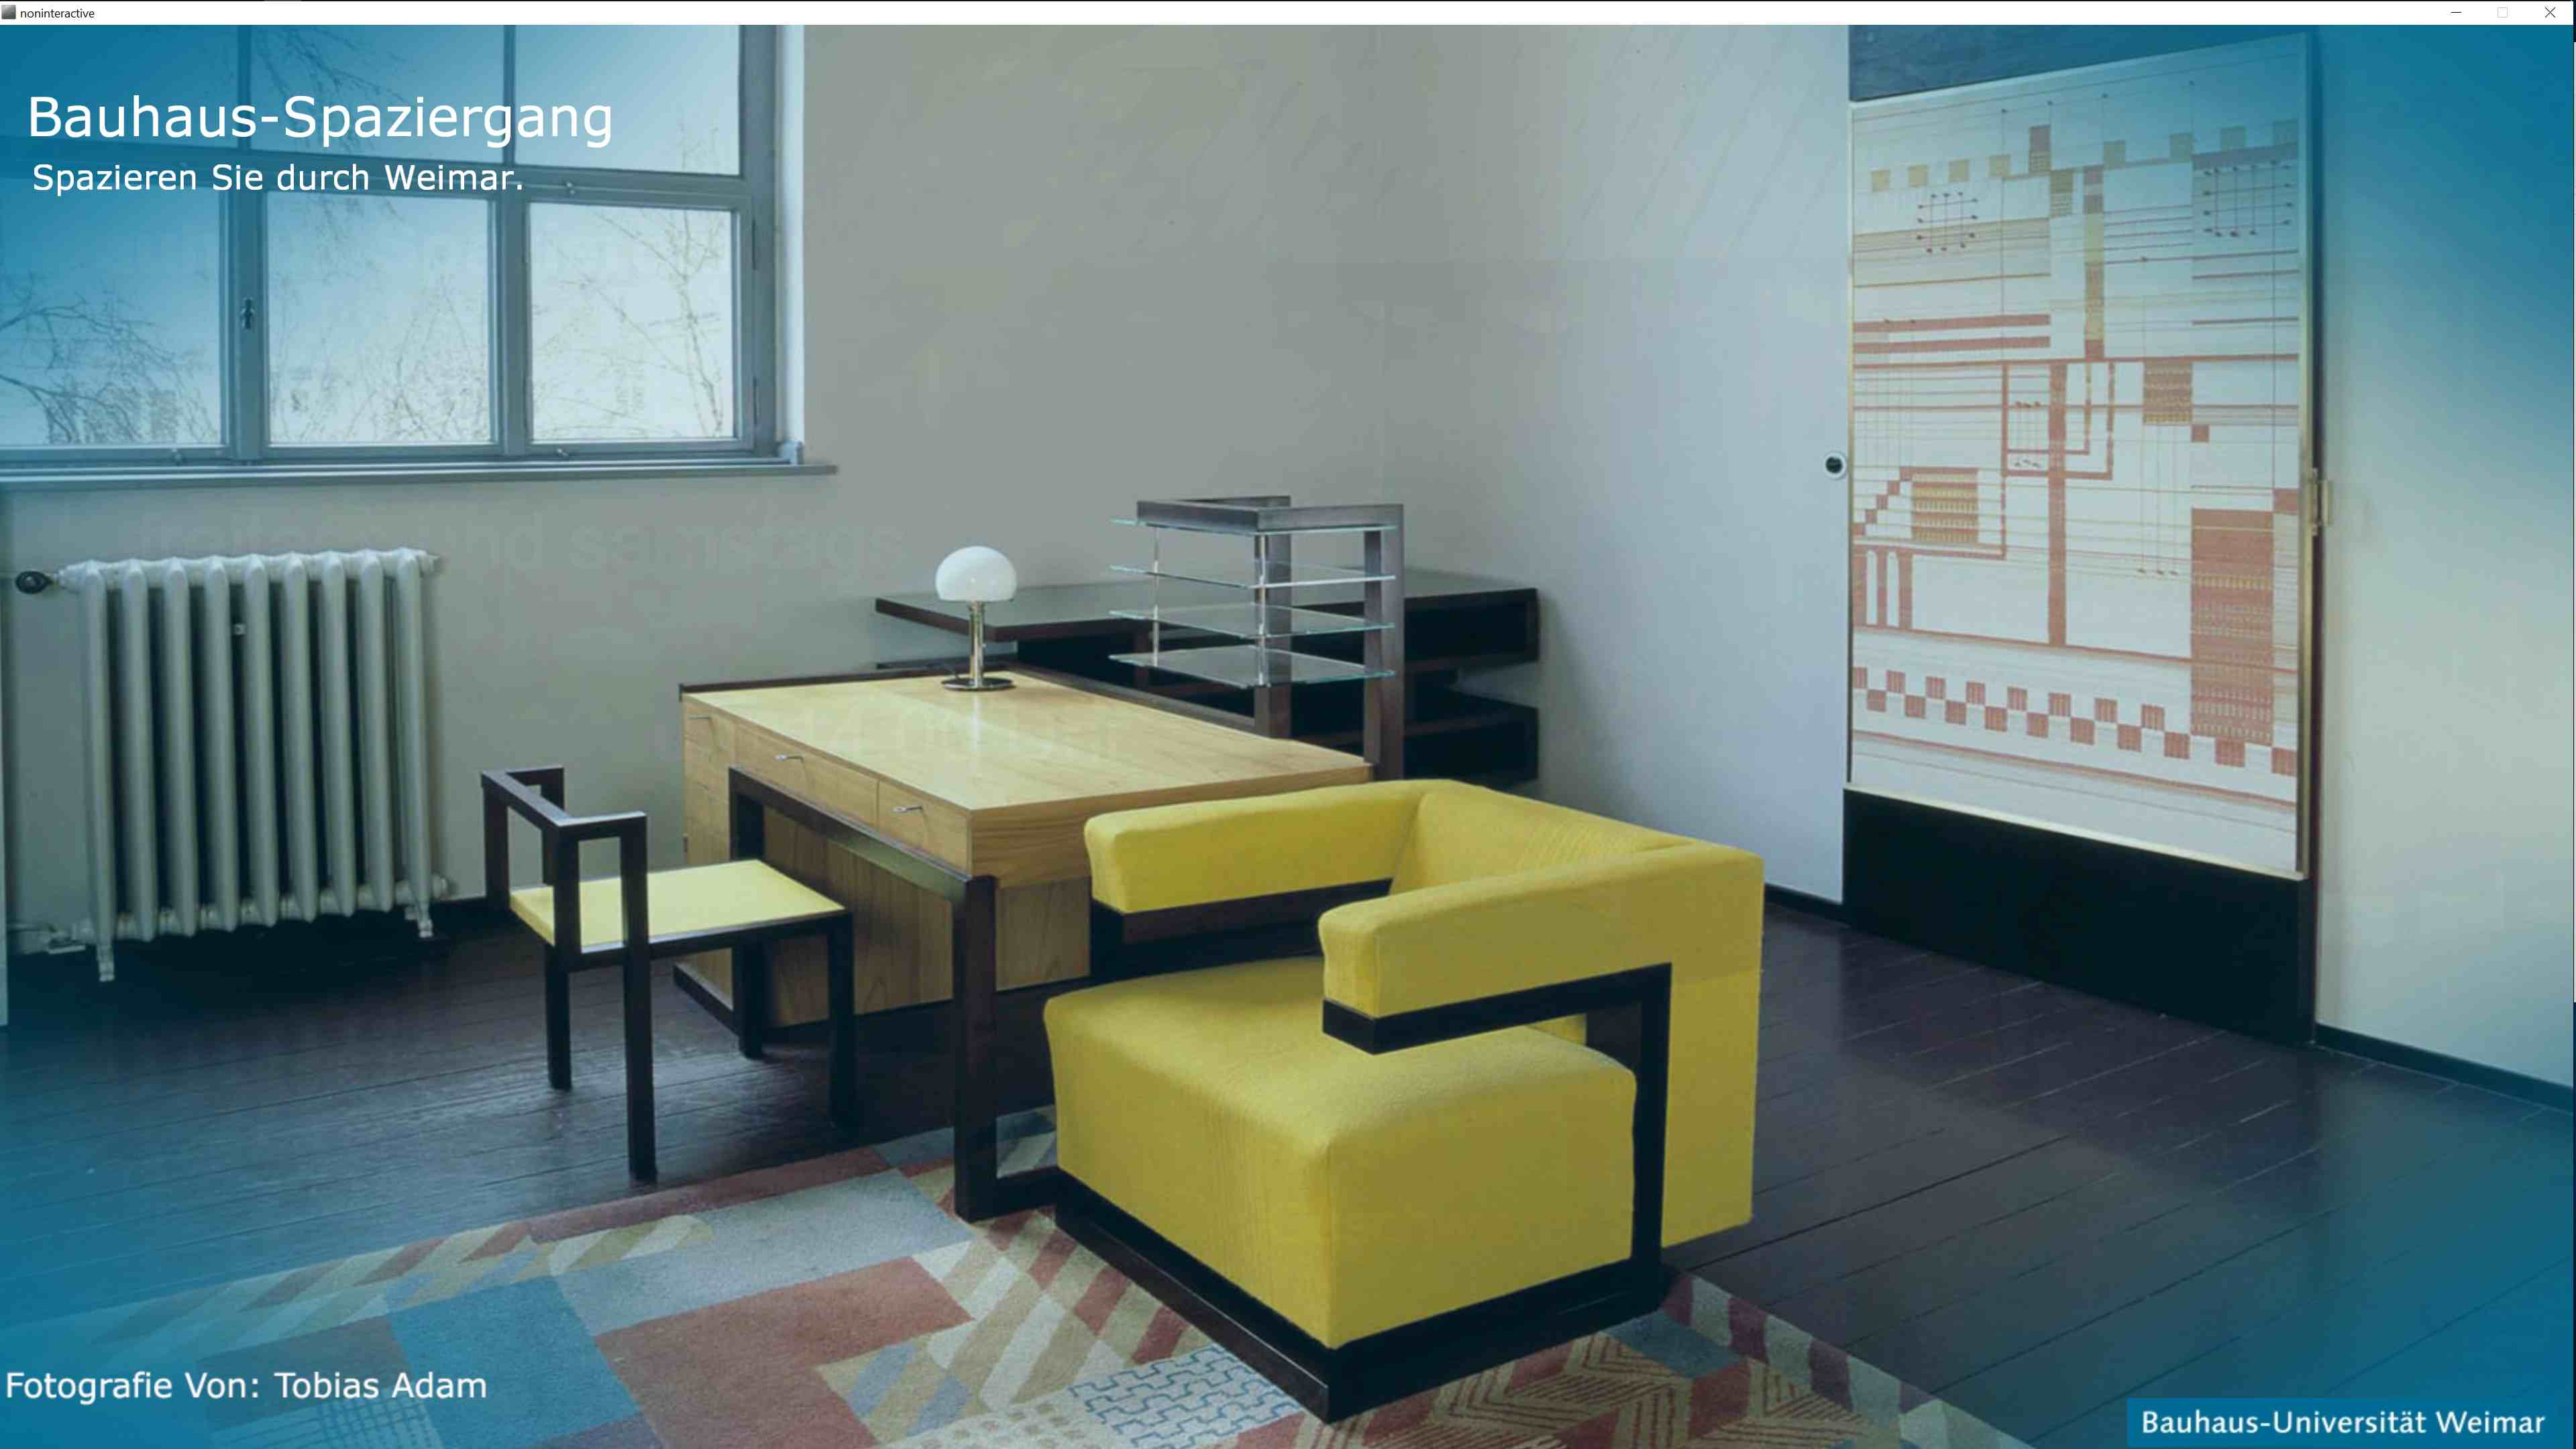
\includegraphics[width=100mm,height=50mm]{Figures/7/initialpage}
    \caption{Initial interface of advertisement: The picture shown is the \emph{Gropius walter} room, and the Event name on the upper left side, and the Bauhaus University logo at the bottom right.}%
    \label{fig:adInitialpage}%
\end{figure}


\begin{figure}[H]
    \centering
    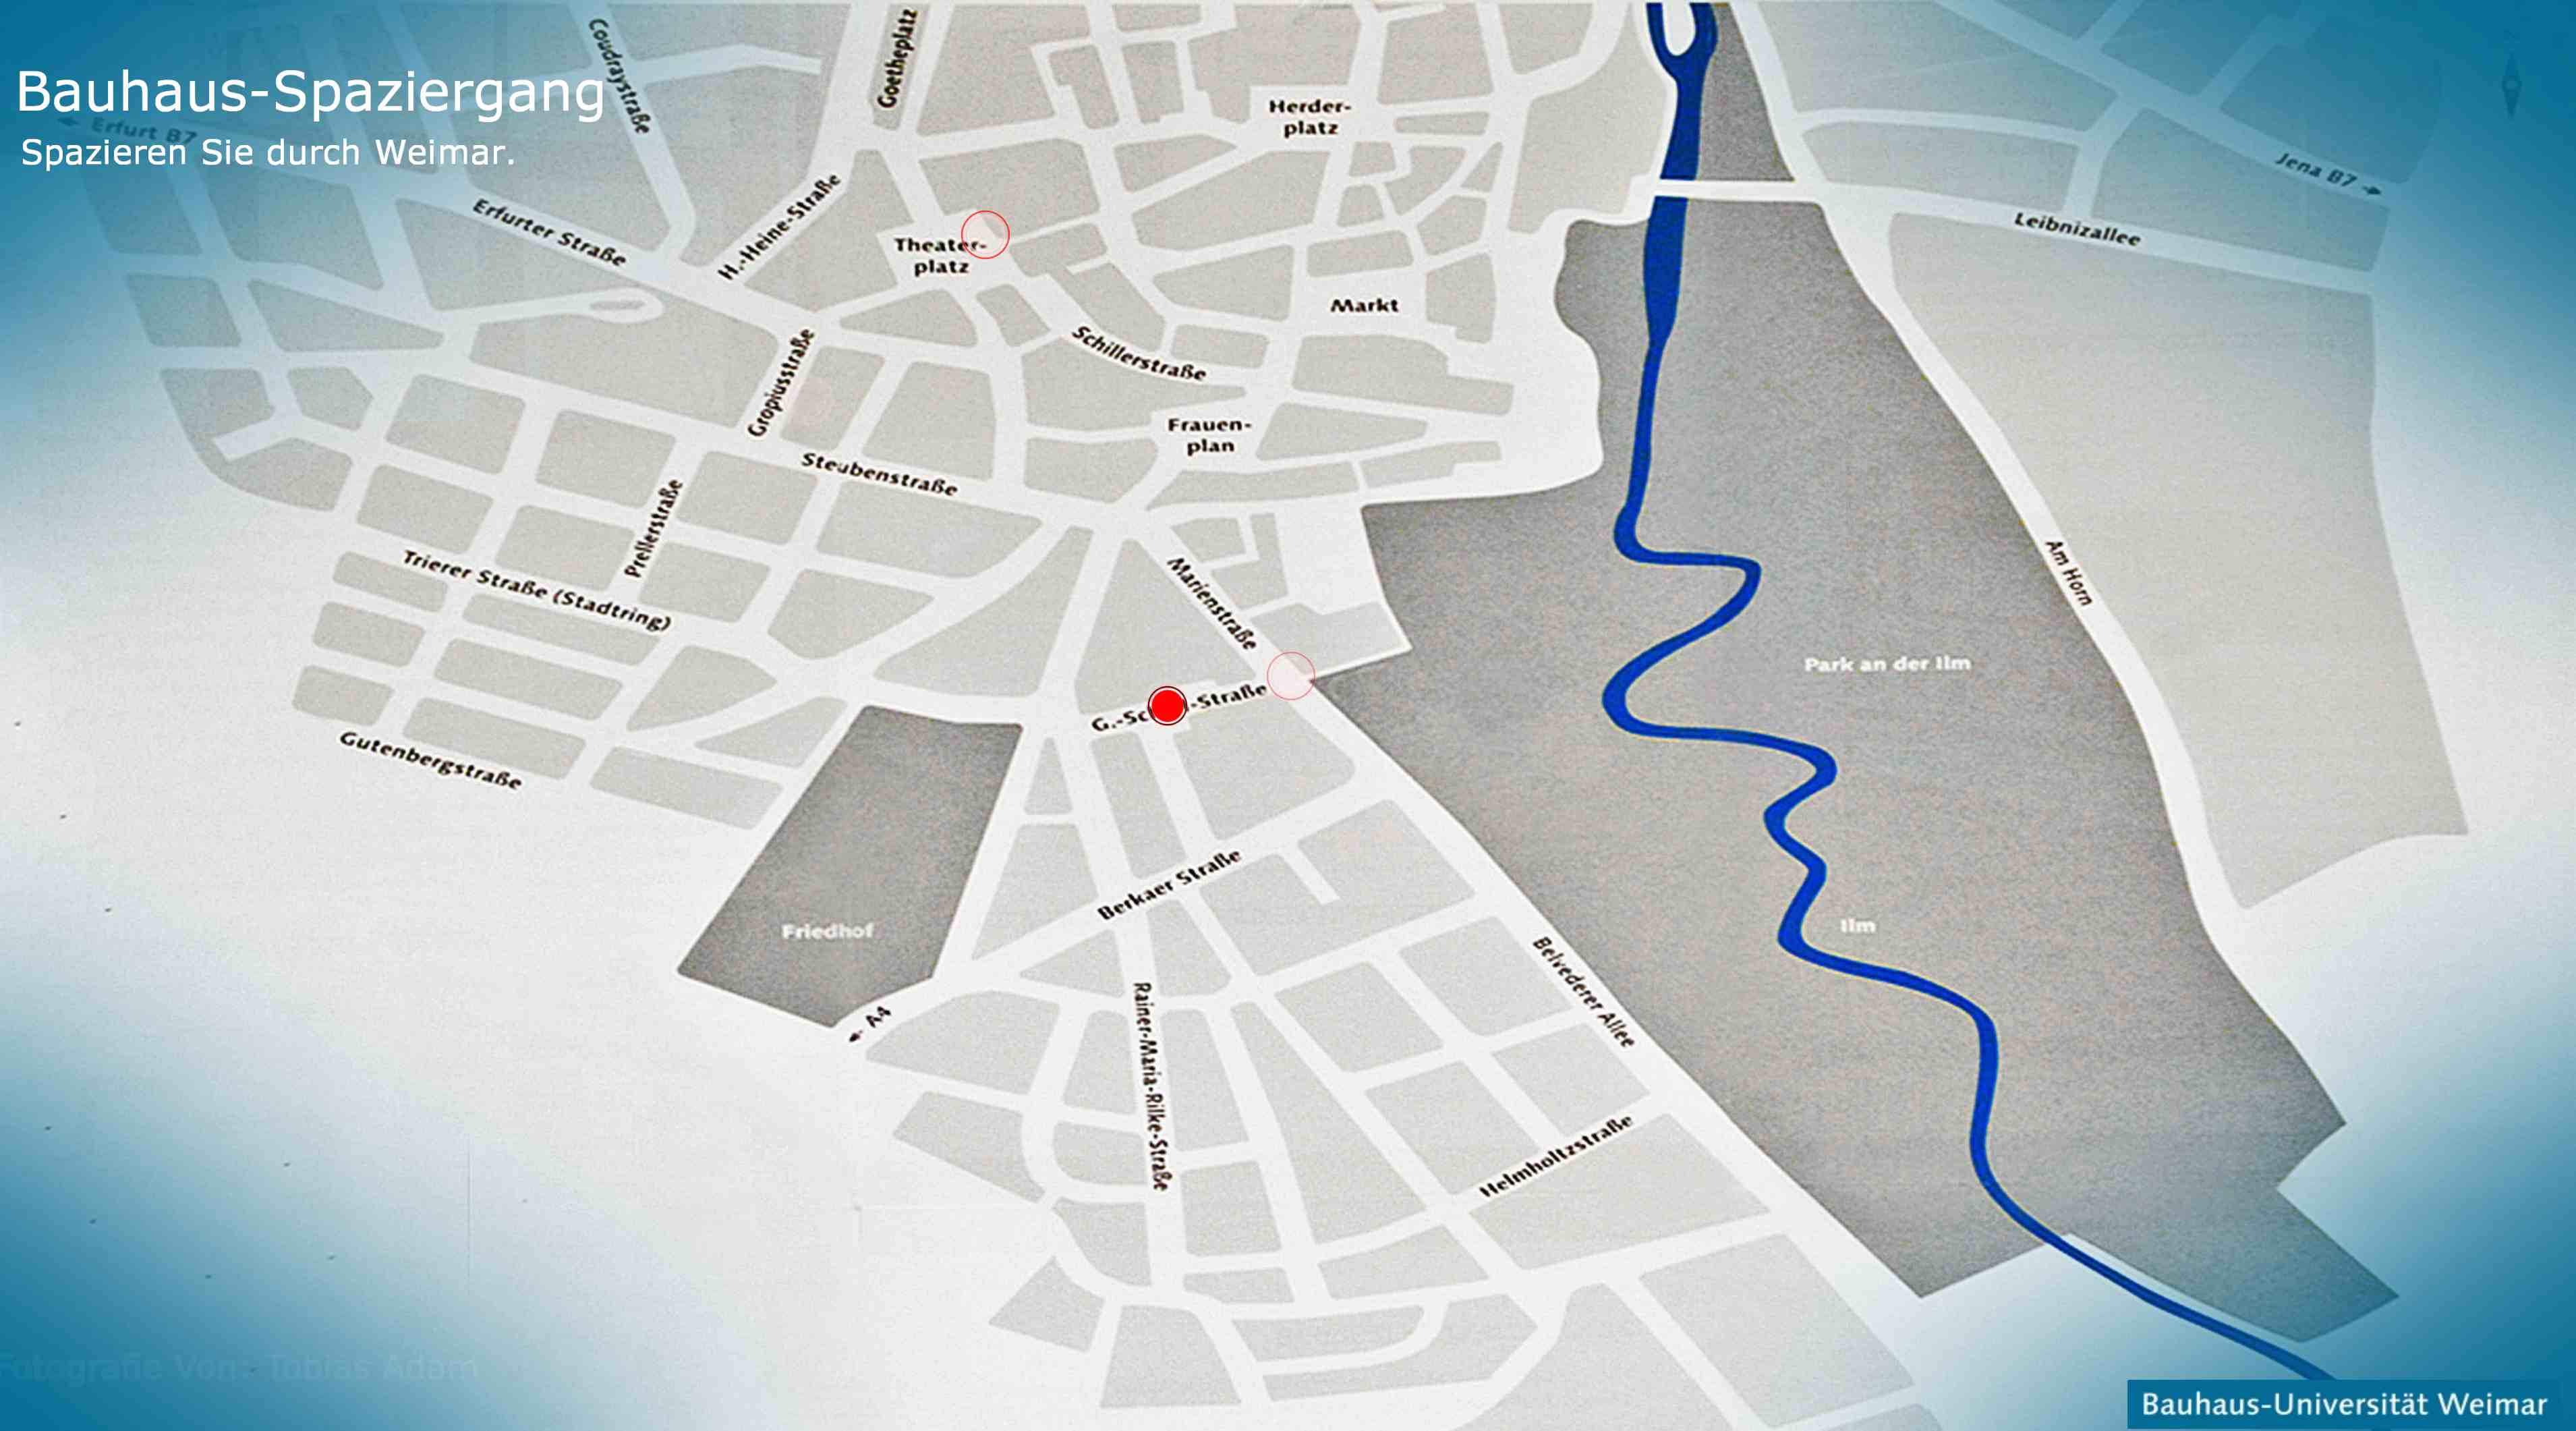
\includegraphics[width=100mm,height=50mm]{Figures/7/map}
    \caption{Second Interface: This is map of Weimar that has some interest regions shown on the top of the map. Those regions are blinking to signal the users.}%
    \label{fig:adSecondpage1}%
\end{figure}


\begin{figure}[H]
    \centering
    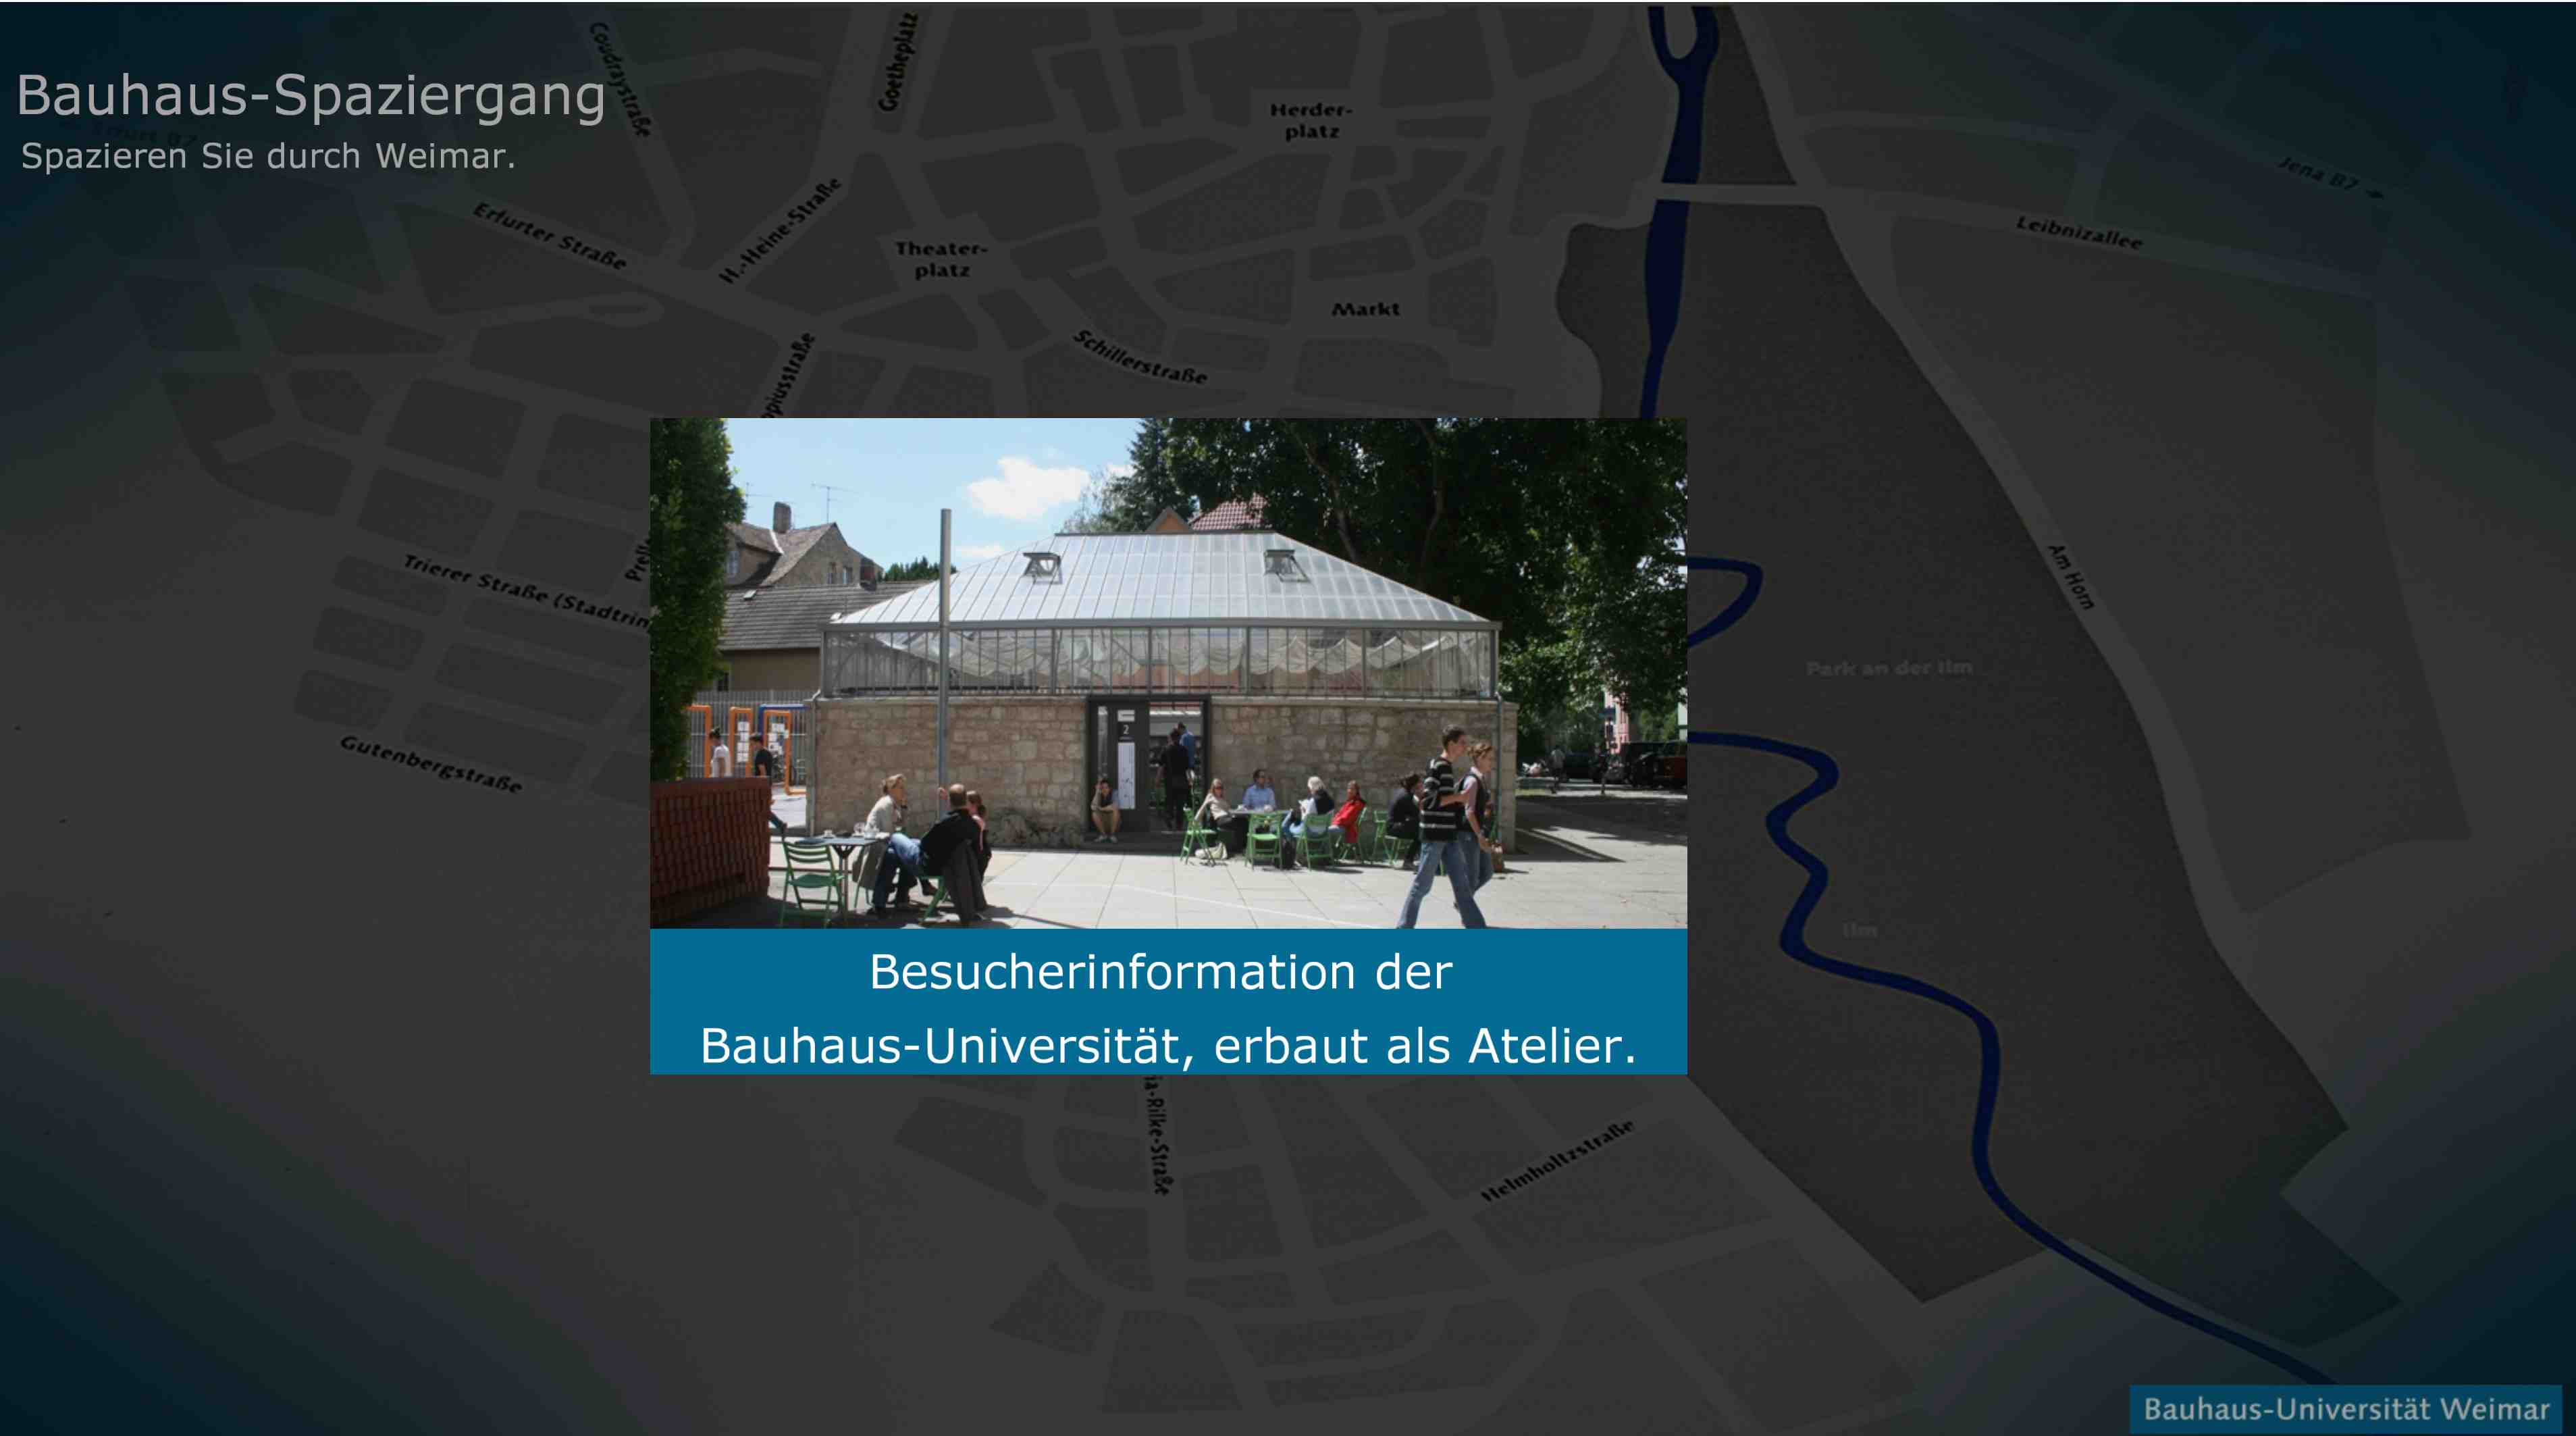
\includegraphics[width=100mm,height=50mm]{Figures/7/enlarged_pic}
    \caption{Second interface: Before the image is shown on the map, first the picture is animated to become enlarged then the picture is resized to fit on the map.}%
    \label{fig:adSecondpage2}%
\end{figure}


\begin{figure}[H]
    \centering
    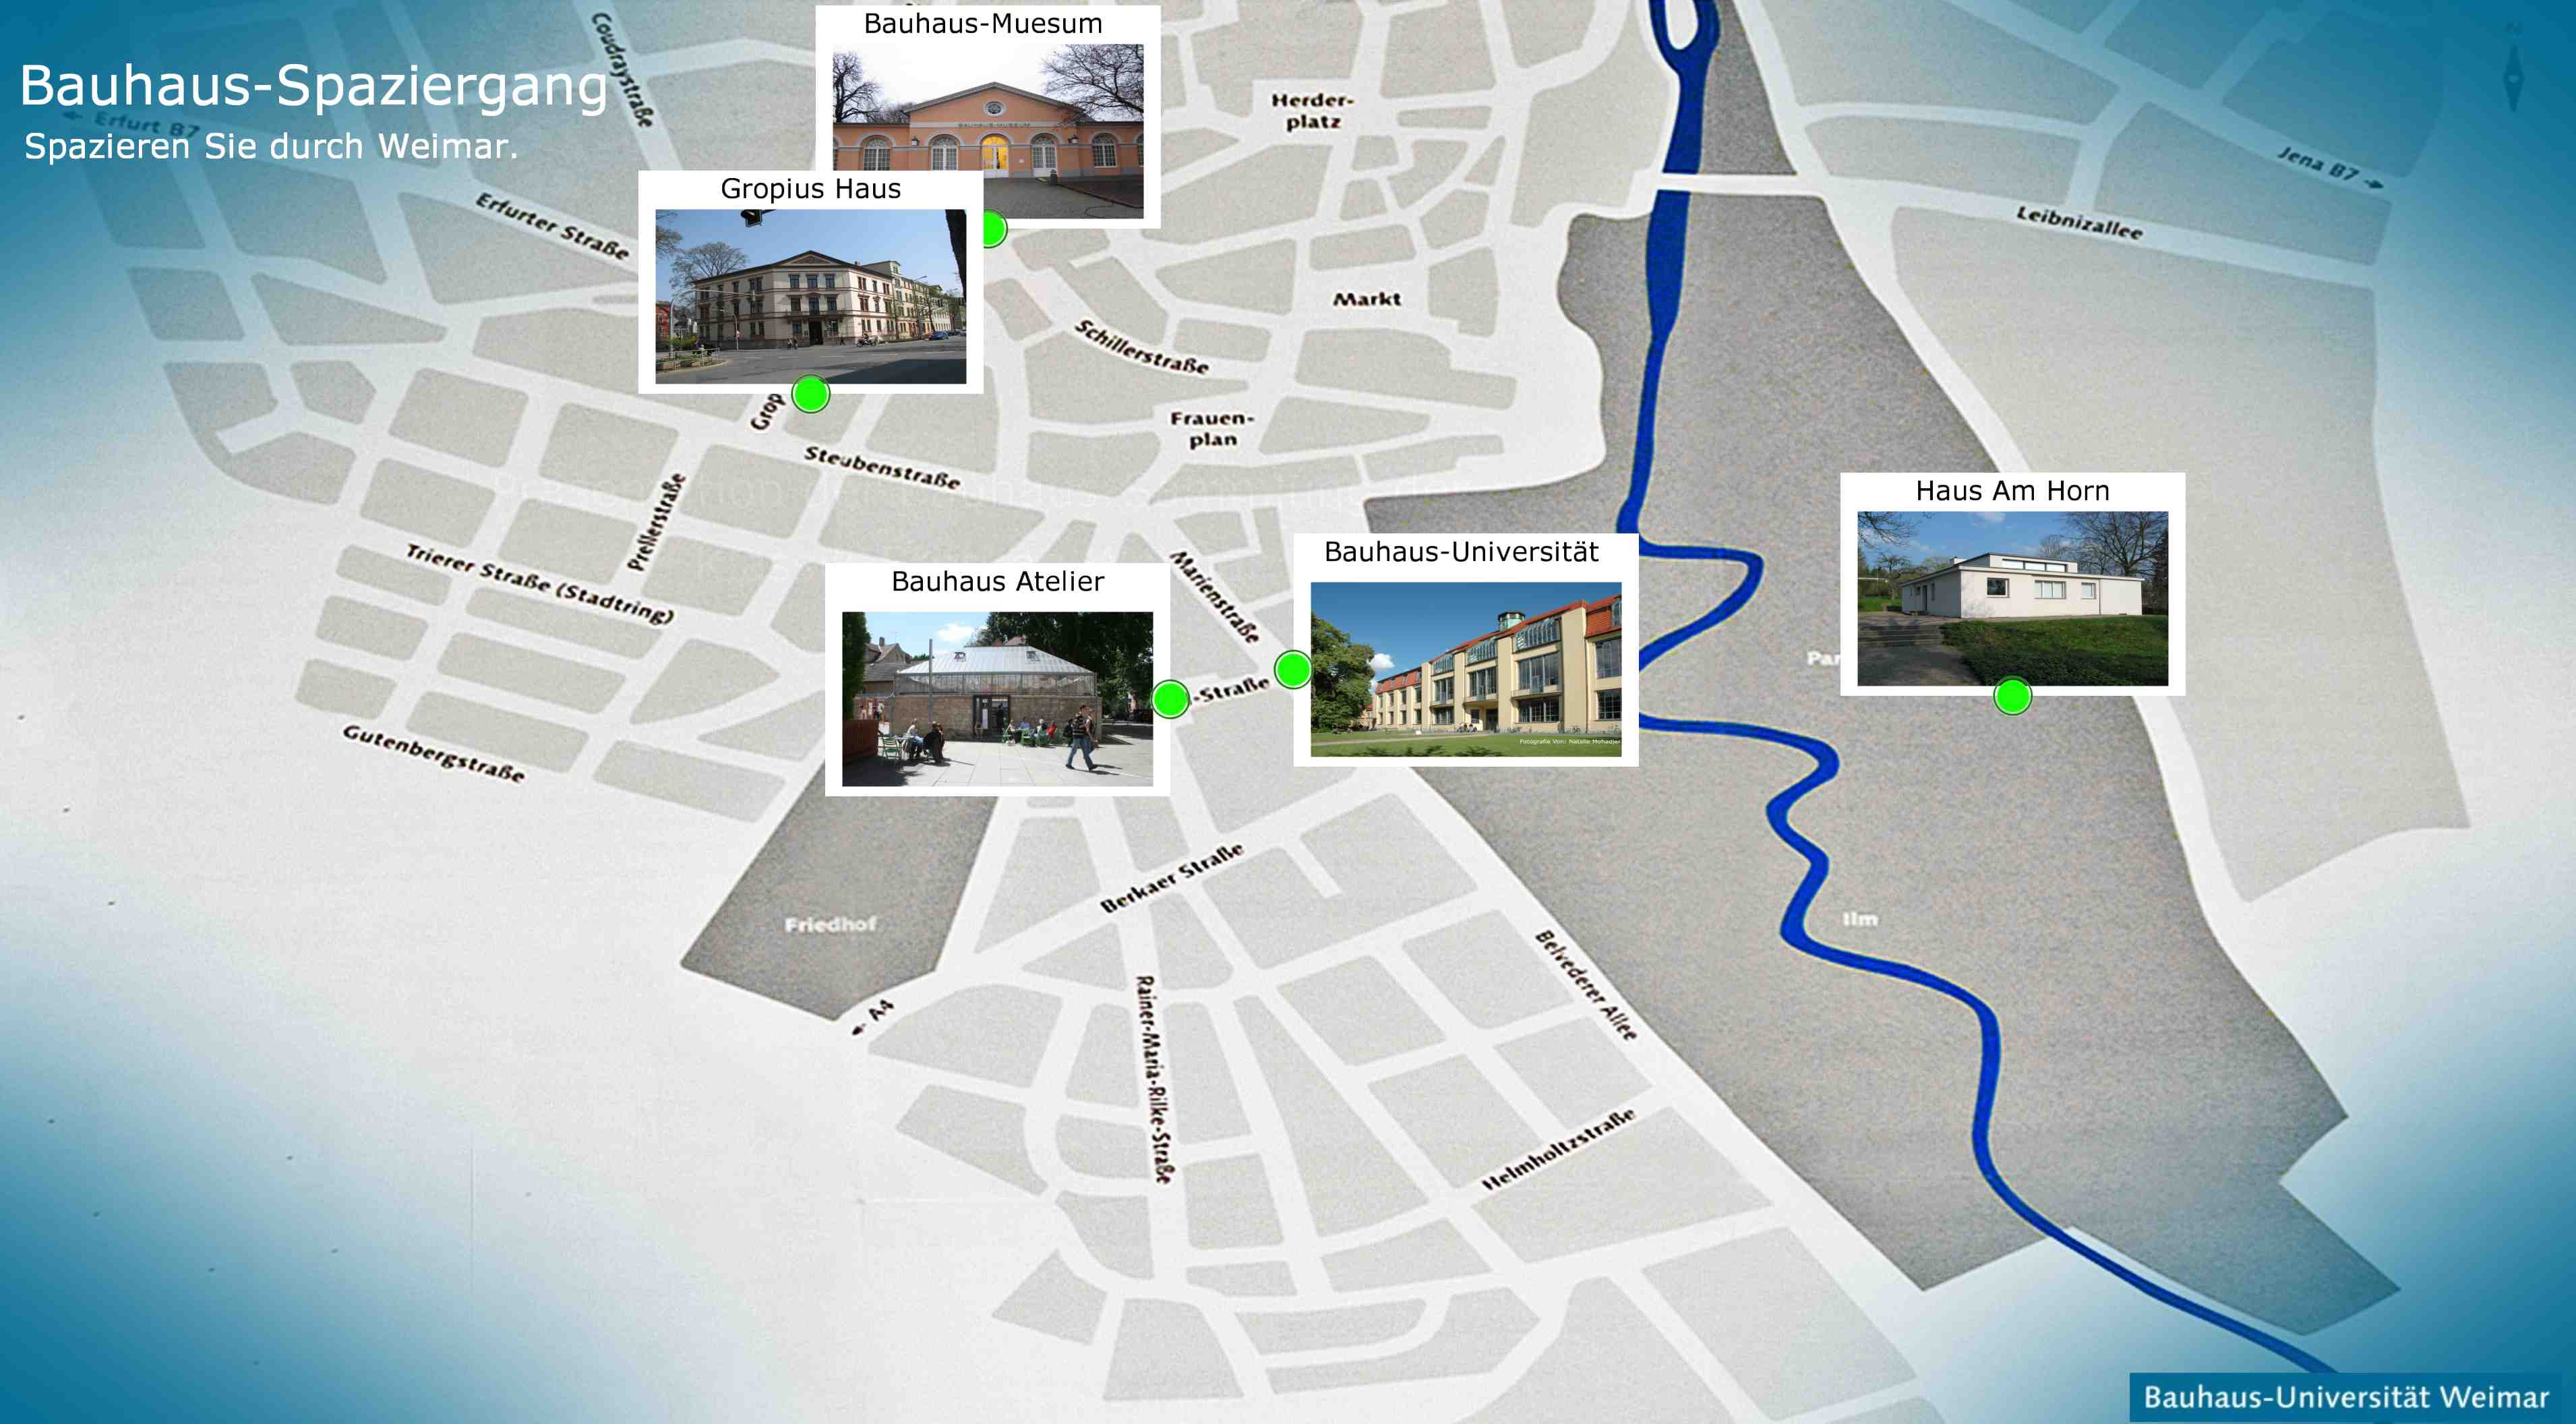
\includegraphics[width=100mm,height=50mm]{Figures/7/map_pictures}
    \caption{Second interface: This shows a map with the picture elements, each picture contains a name}%
    \label{fig:adSecondpage3}%
\end{figure}

\begin{figure}[H]
    \centering
    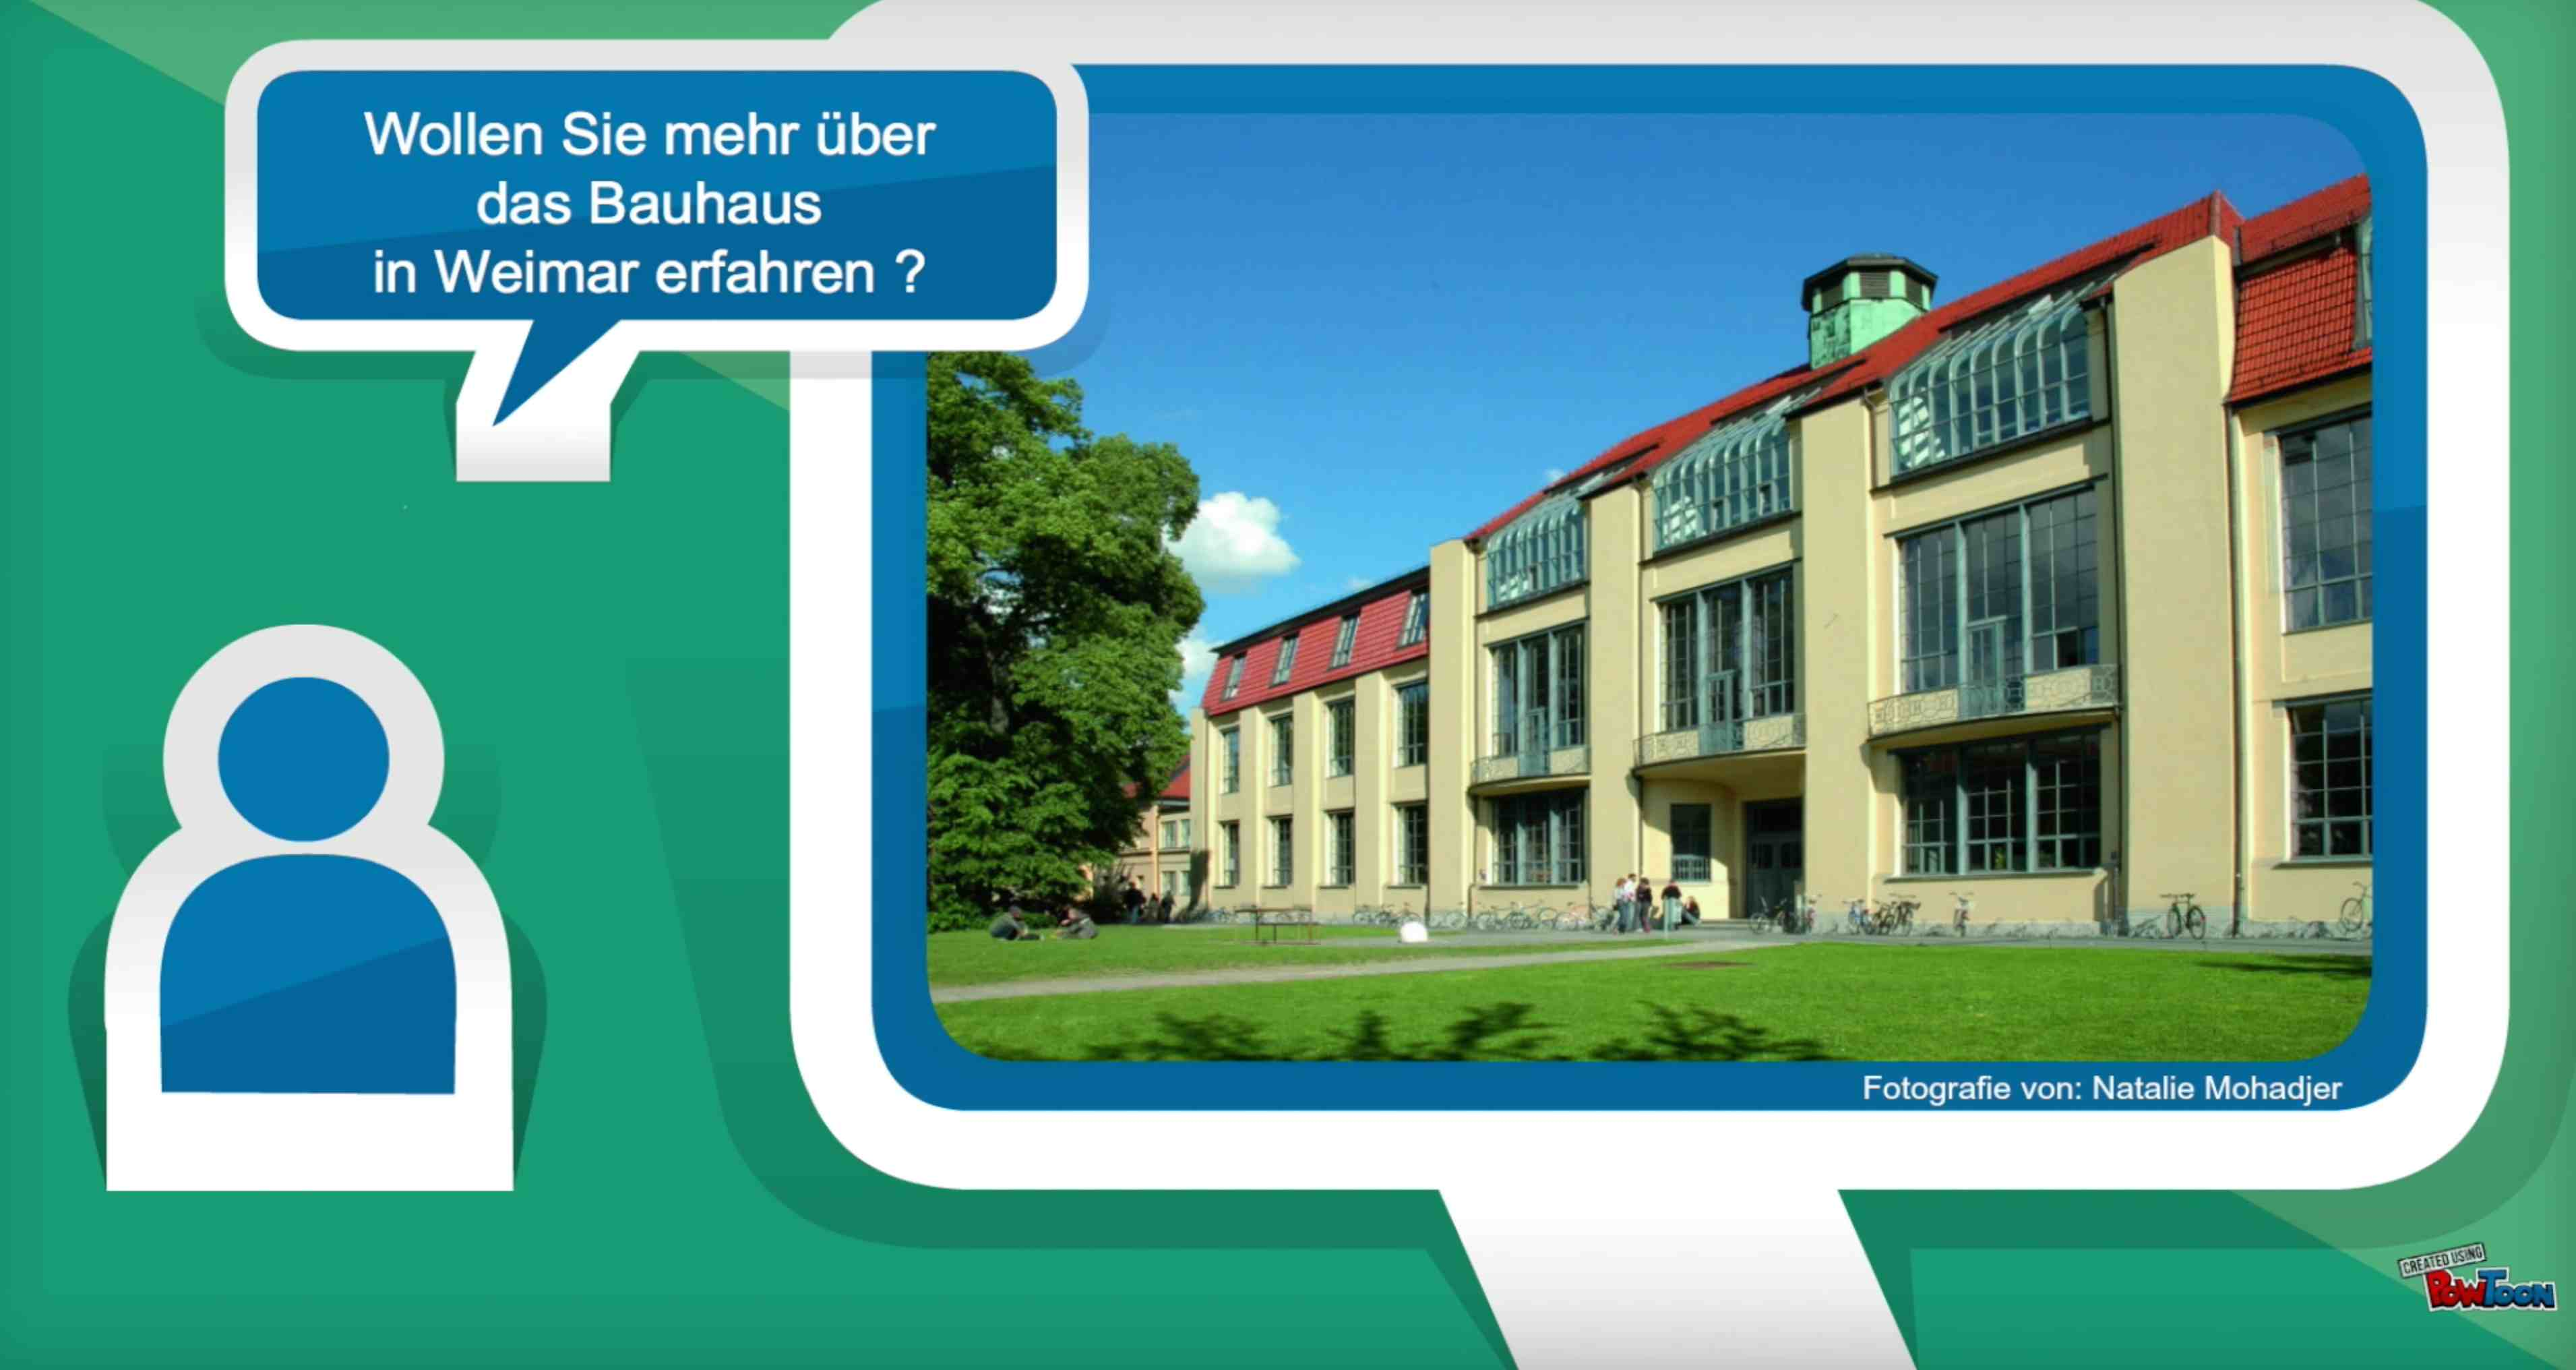
\includegraphics[width=100mm,height=50mm]{Figures/7/ad_first}
    \caption{Third interface: In this interface the video is being played, this picture is a screenshot of one of the frames of the video}%
    \label{fig:adthirdpage1}%
\end{figure}


\begin{figure}[H]
    \centering
    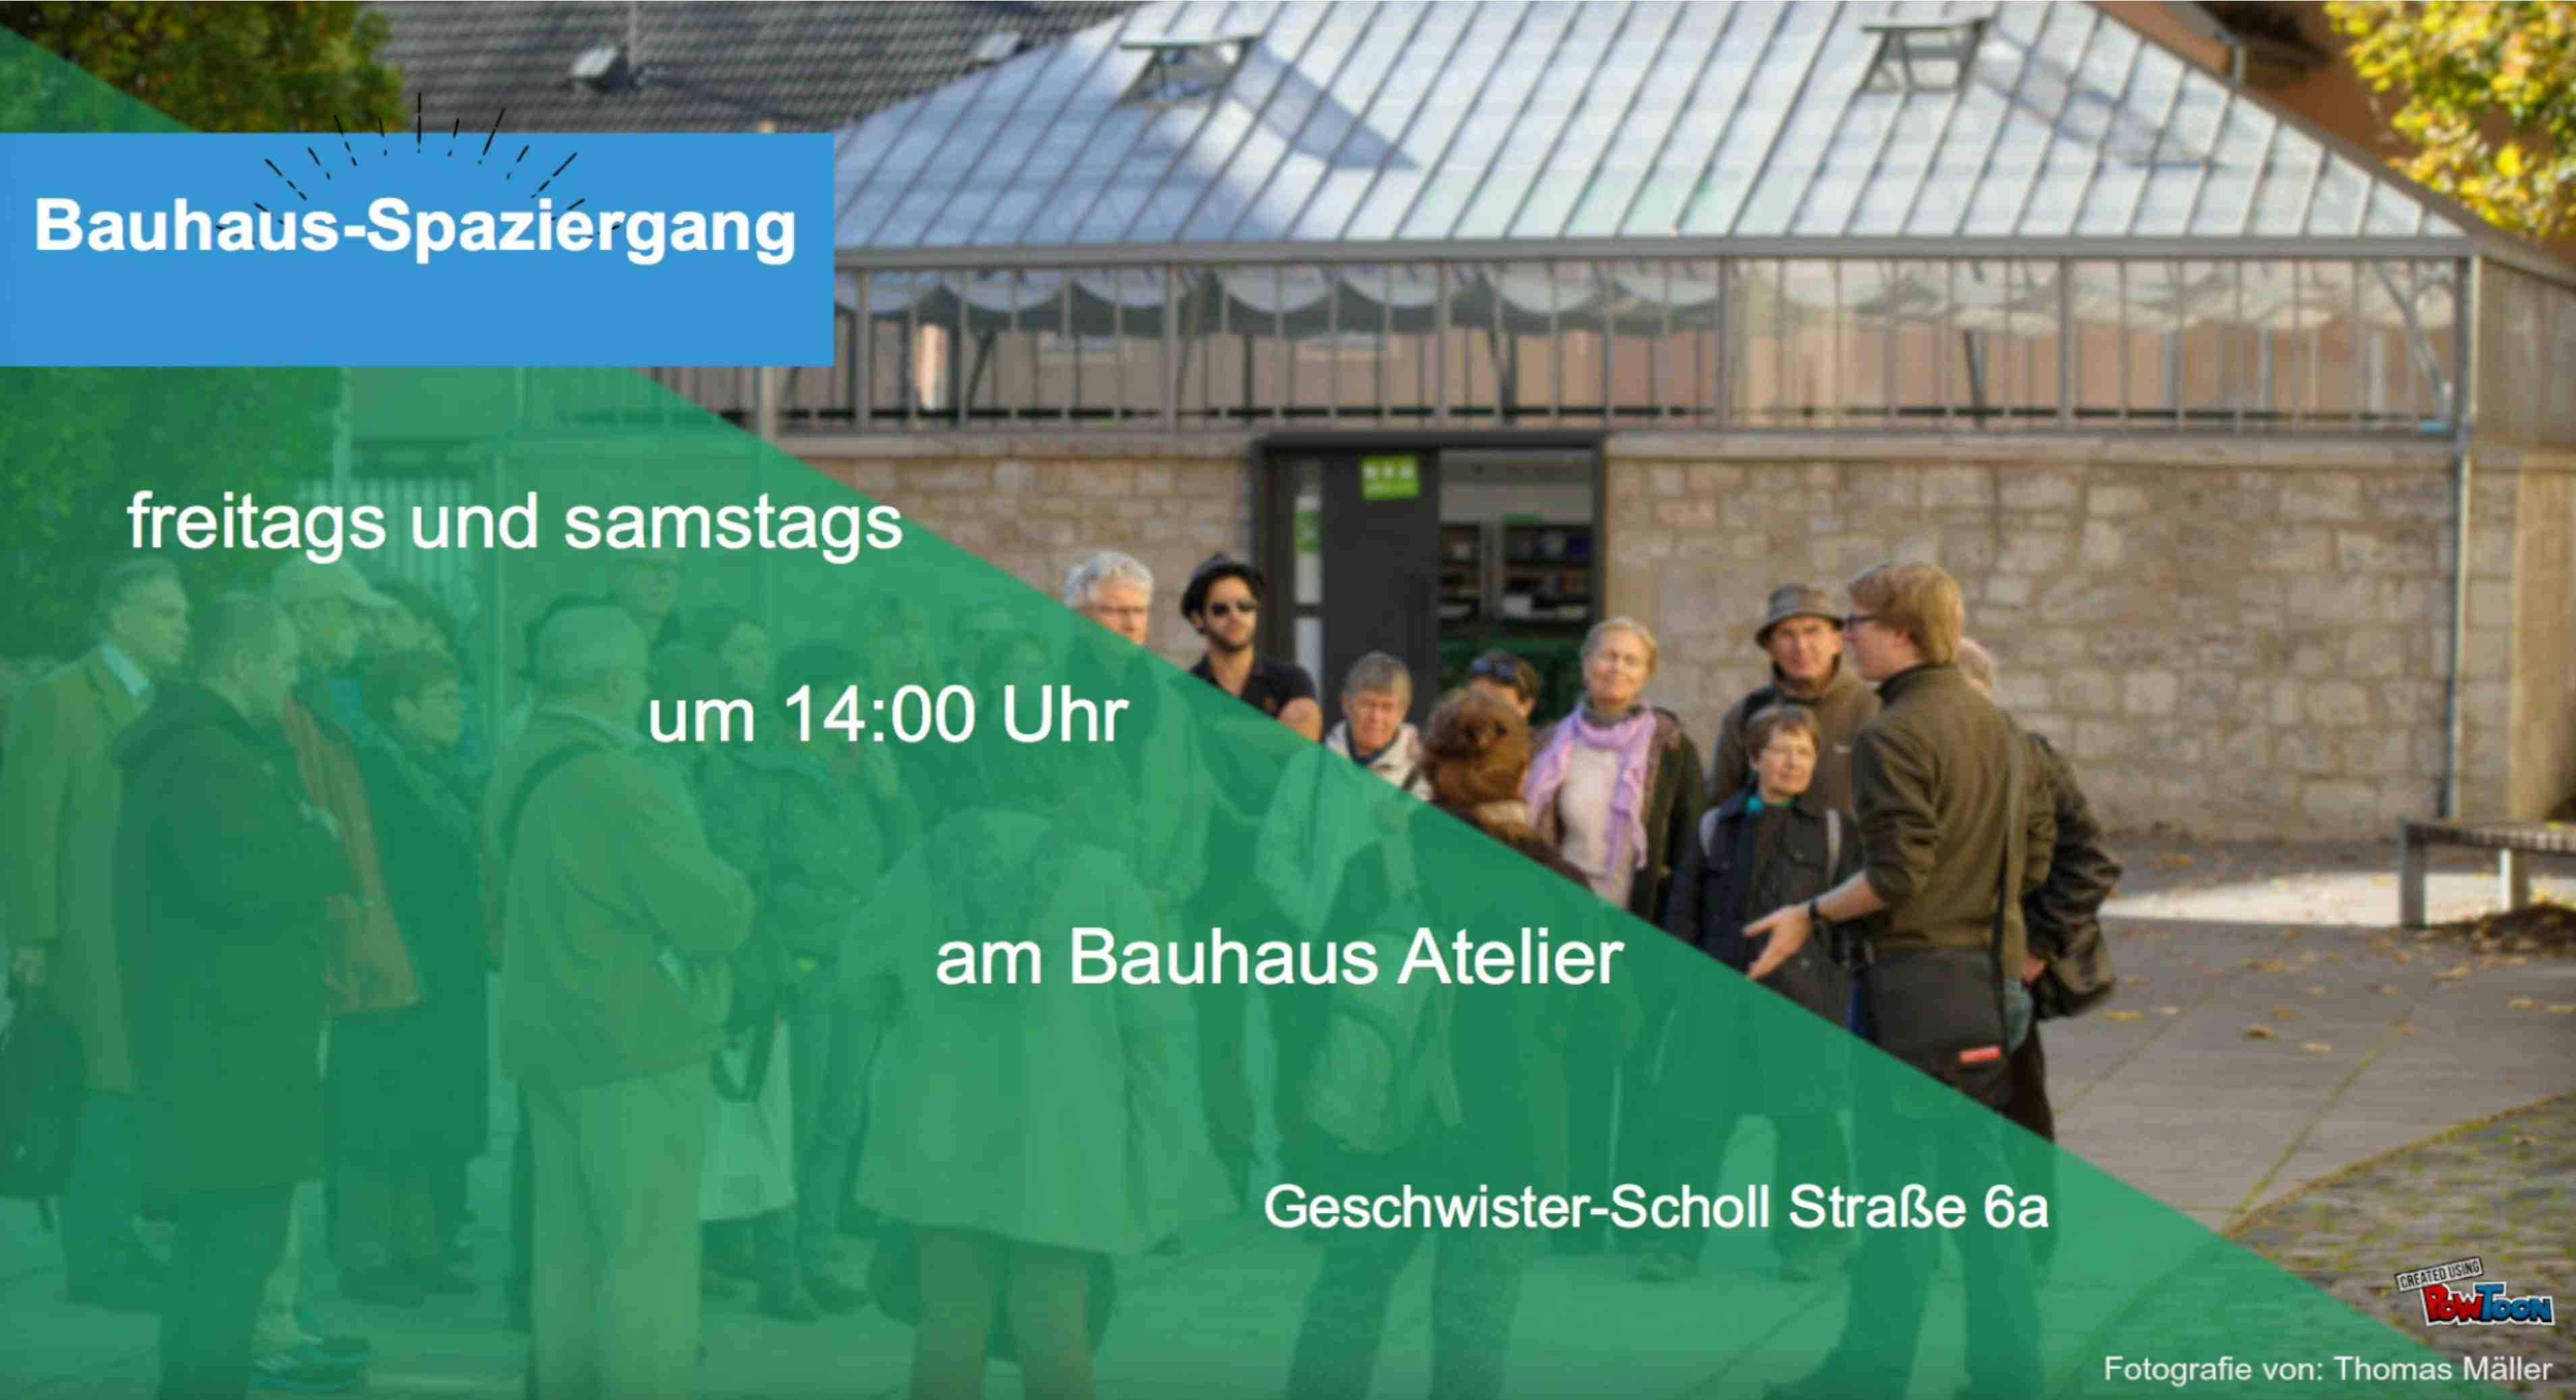
\includegraphics[width=100mm,height=50mm]{Figures/7/ad_last}
    \caption{Third interface: This is the last frame of the video that shows information about how and where to join the Bauhaus Walk.}%
    \label{fig:adthirdpage2}%
\end{figure}

Please watch the complete animation stored in DVD. 


\subsection{Advertisement video}
The advertisement video was created in powtoon \cite{powtoon} with a free version account, to see the full advertisement video visit bellow link.\\ \url{https://www.youtube.com/watch?v=-y1Dbz6E6bU&feature=youtu.be}

\subsection{Hardware setup}
The bellow setup is the hardware setup for the advertisement. The same setup is used for all three weeks.

\begin{figure}[H]
    \centering
    \includegraphics[width=100mm,height=70mm]{Figures/7/Physical_setup}
    \caption{Hardware setup}%
    \label{fig:hardwaresetup}%
\end{figure}


\hilight{put the picture of the screen here}

\begin{figure}[H]
    \centering
    \includegraphics[width=100mm,height=70mm]{Figures/7/Physical_setup}
    \caption{Picture}%
    \label{fig:hardwaresetup}%
\end{figure}



\subsection{Non-Interactive application}
As can be understood the application is not influenced by the passers-by but triggers automatically, it automate through whole three phases (Initial screen, Map screen and video screen) and at the same time records colored image frames using Kinect Camera.


\subsubsection{Flowchart Diagram}

\begin{figure}[H]
    \centering
    \includegraphics[width=100mm,height=90mm]{Figures/7/Non-interactive/flow_chart_diagram}
    \caption{Non-interactive Flowchart diagram}%
    \label{fig:non_inter_flowchart}%
\end{figure}

\newpage
\subsection{Body Interactive application}
This method allows participants to interact with using body on the map, in this case exploring the interest points on the map by moving physically (forward, backward, right and left) in front of the screen in order to move their silhouette and reach to the interest regions.

As discussed earlier there are three phases of the application, First Interface, second interface and then the advertisement video. The first two interfaces are interactive as described bellow.

\subsubsection{First interface}
This interface is basically the attraction attention and call-to-action interface, as you can see bellow there is someone standing in front of the screen and the interface calls him to come near. This area also has alert message on the top right area of the screen and alerts the participant if they move away from the camera range, in this example the person is standing but there is also the second person but got immediately untracked and the system pops that message to raise his hand to be tracked again.
\begin{figure}[H]
    \centering
    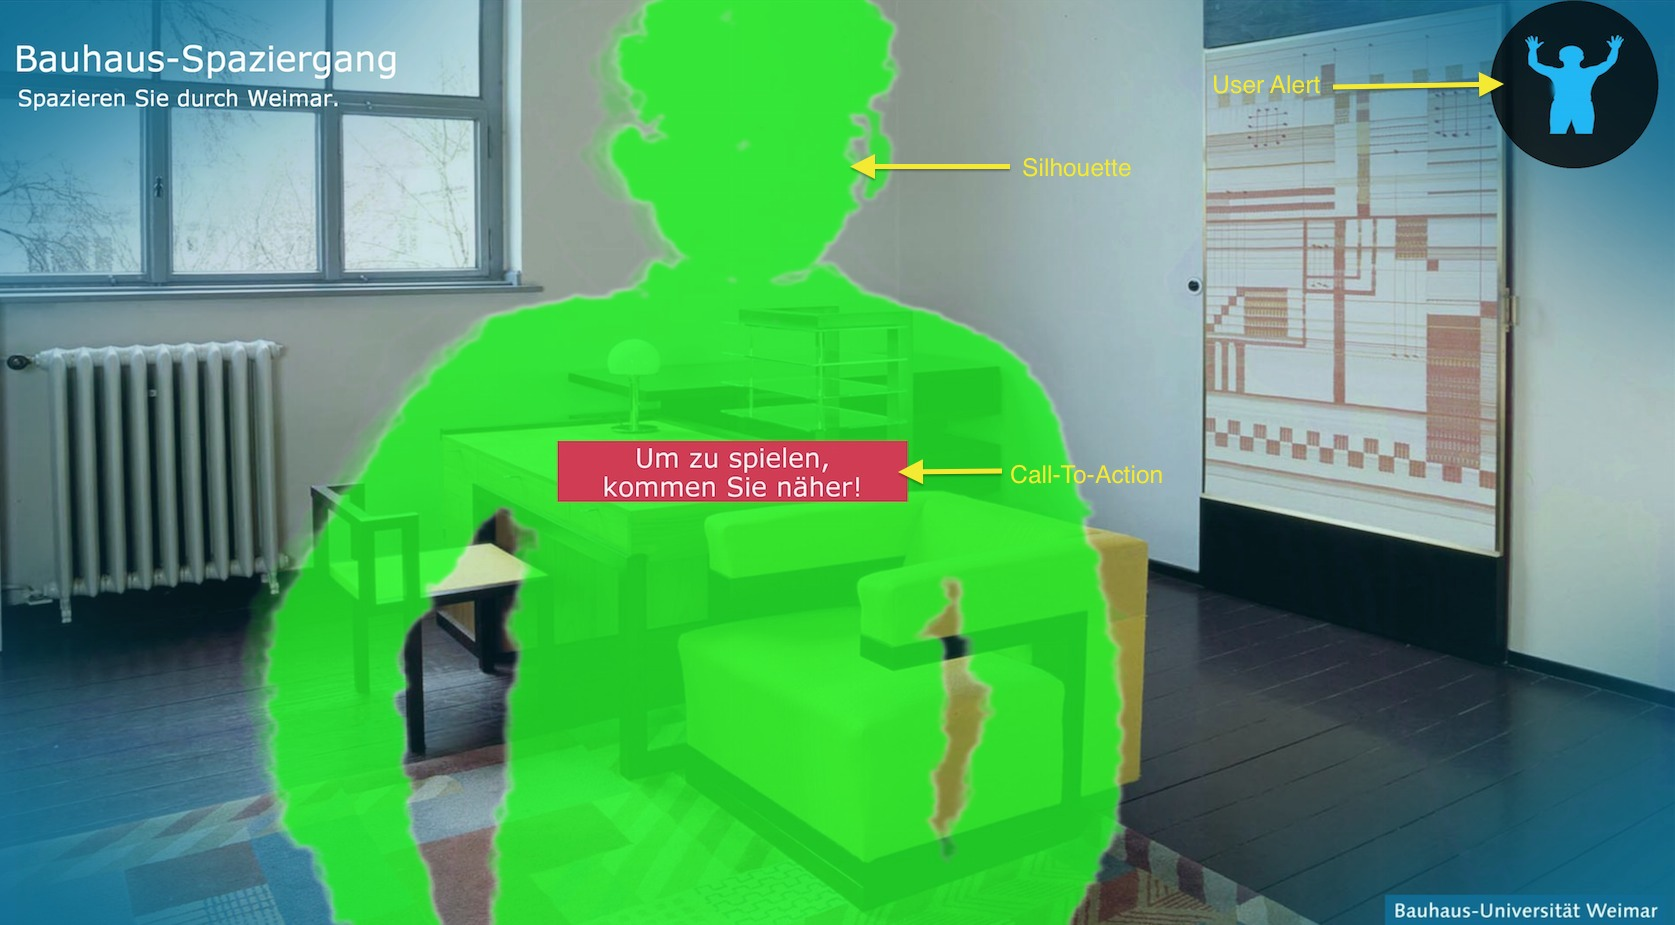
\includegraphics[width=100mm,height=60mm]{Figures/7/body_interactive/first_interface}
    \caption{\textbf{First Interface:} When the person steps in the range of the Camera, his silhouette is projected on the screen with a different color; the application calls the person to come near in order to trigger the game.}%
    \label{fig:body_firstinterface}%
\end{figure}



\subsubsection{Transition to second interfaces}
The transition happens when the person stands close to the screen for more than 3 seconds and the bellow things happen.

\begin{enumerate}
\item Loading animation:\\
  The loading animation is a reaction to the action of the participants, and at the same time participants waits for something to be loaded.
\item Scaling down the silhouette: \\
To walk freely on the map and to give the participant the feeling of walking, the participant's silhouette is scaled down, the scaling happens smoothly frame-by-frame.
\item Show task instruction:  \\
Every interaction has instructions, the instruction is fairly very easy and it is simplified in one sentence to explore locations on the map.
\end{enumerate}



\begin{figure}[!htb]
    \centering
    \subfloat[]{{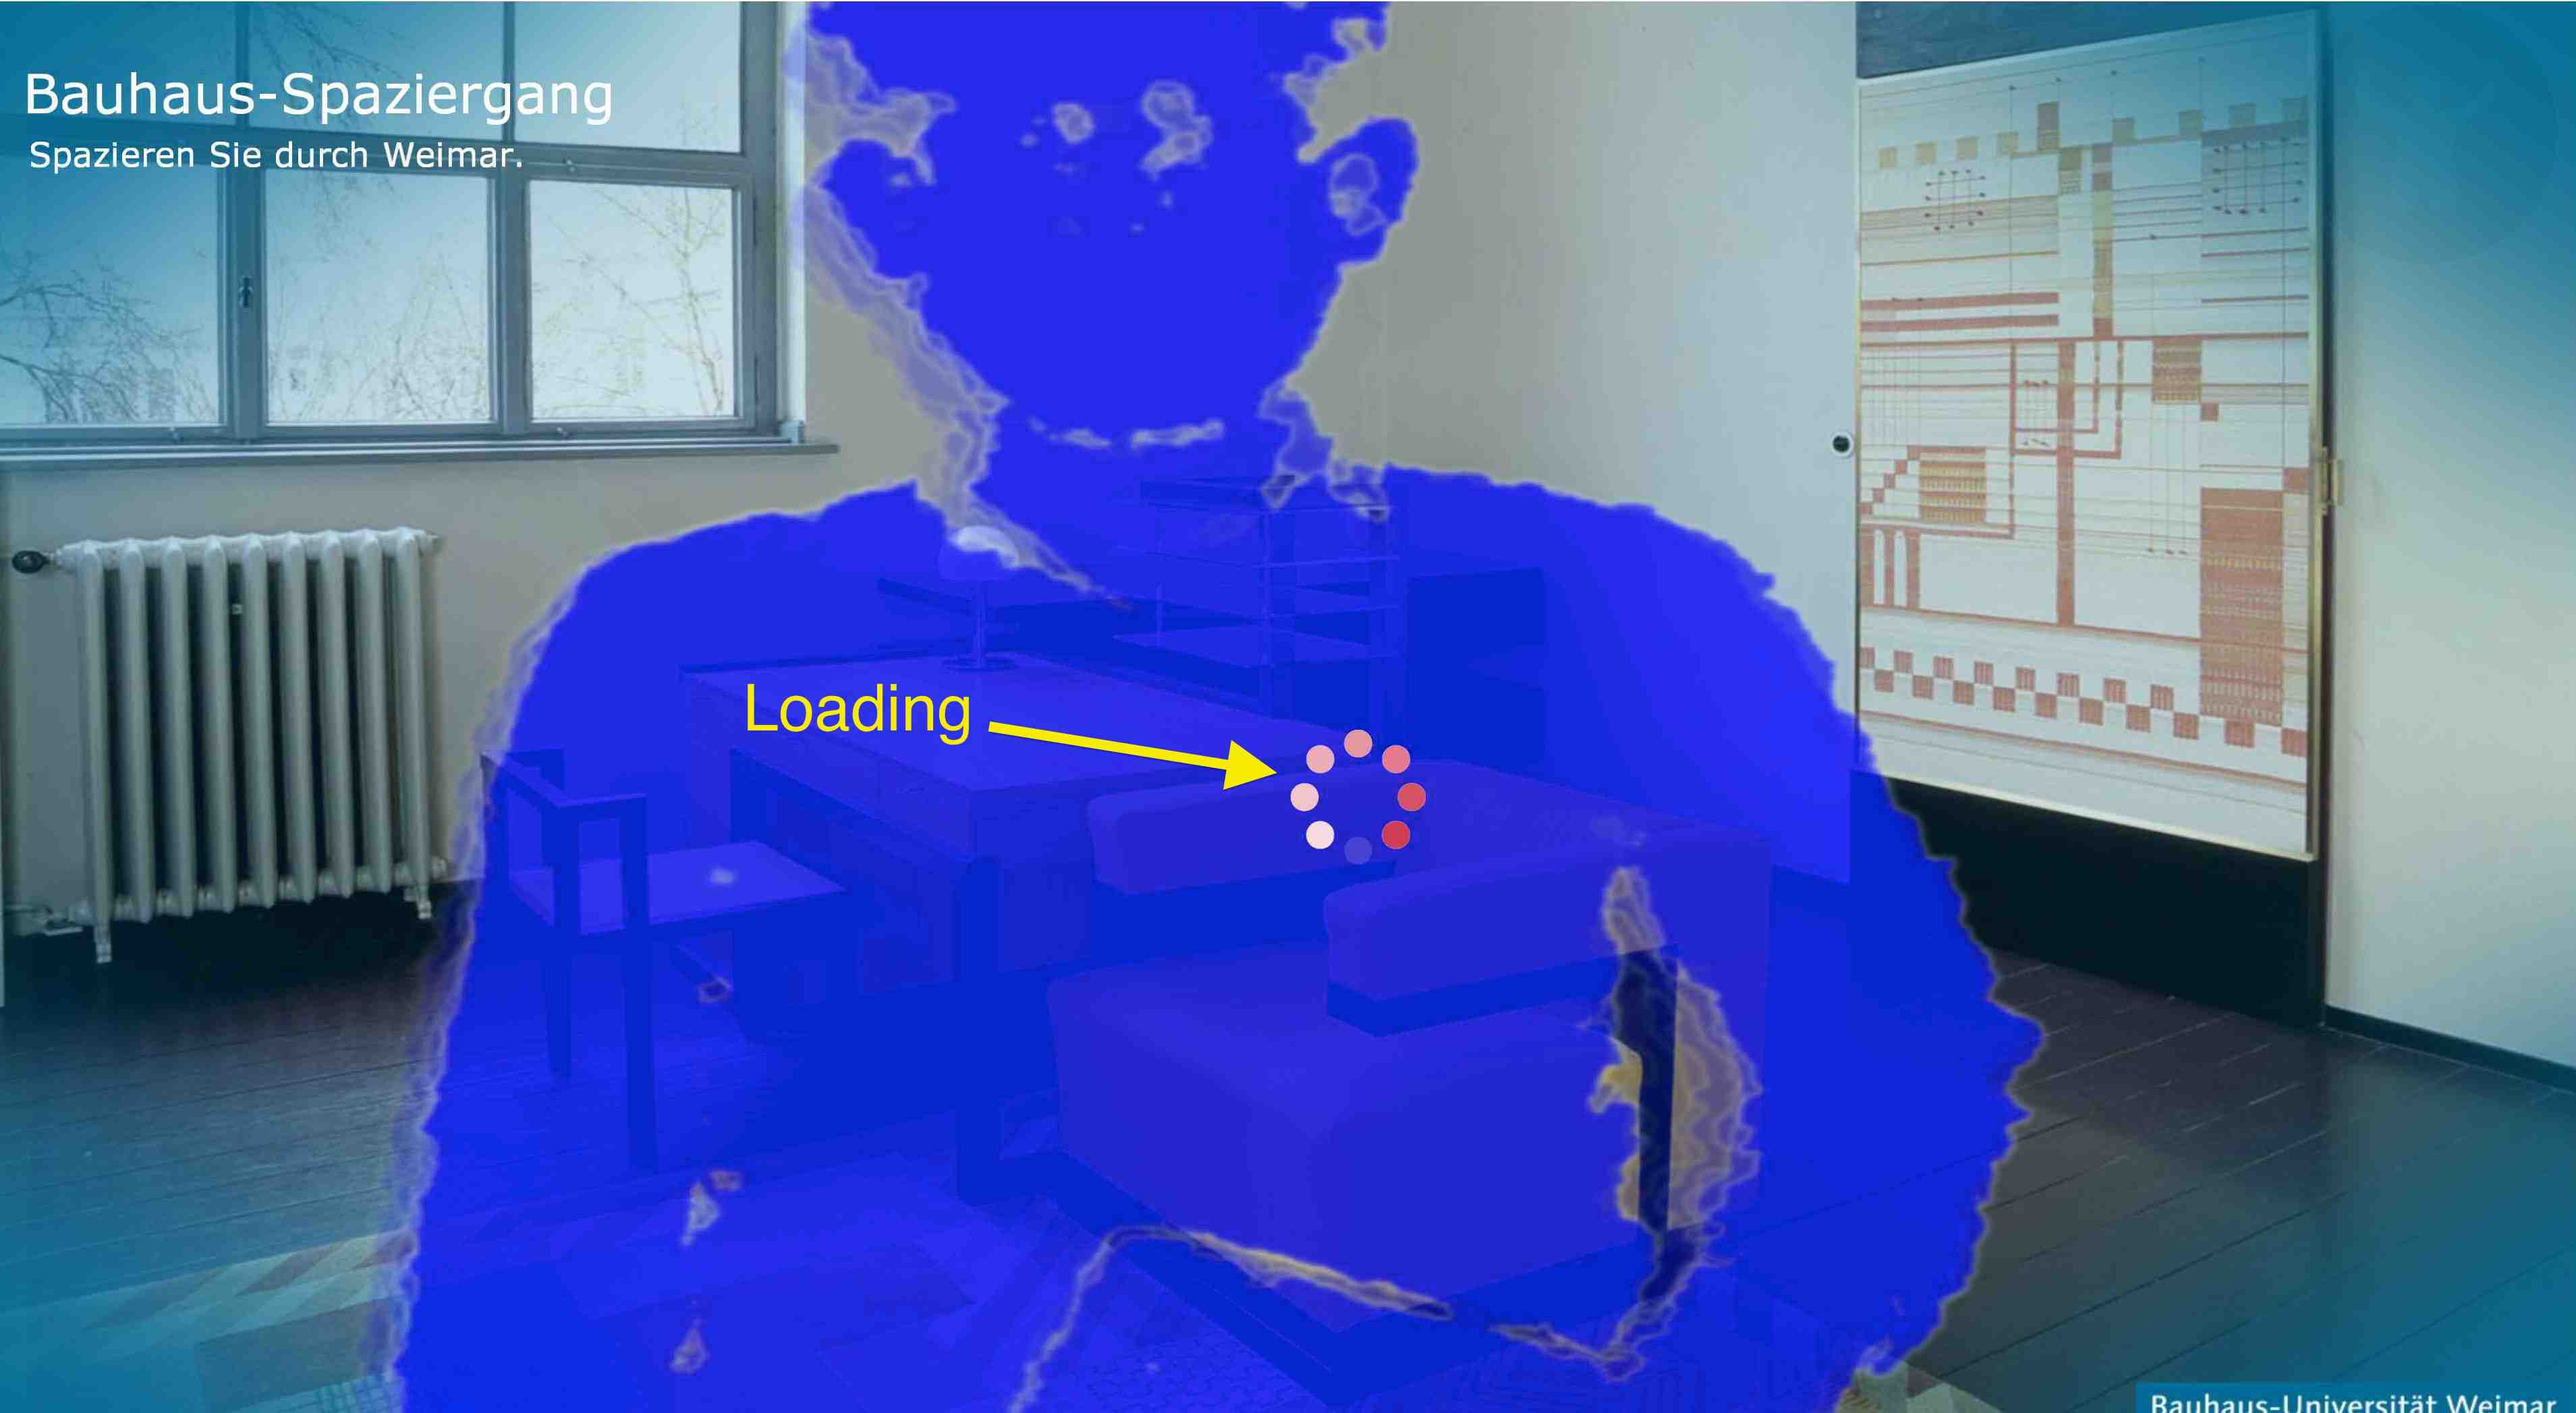
\includegraphics[width=40mm,height=30mm]{Figures/7/body_interactive/loading} }}%
    \subfloat[]{{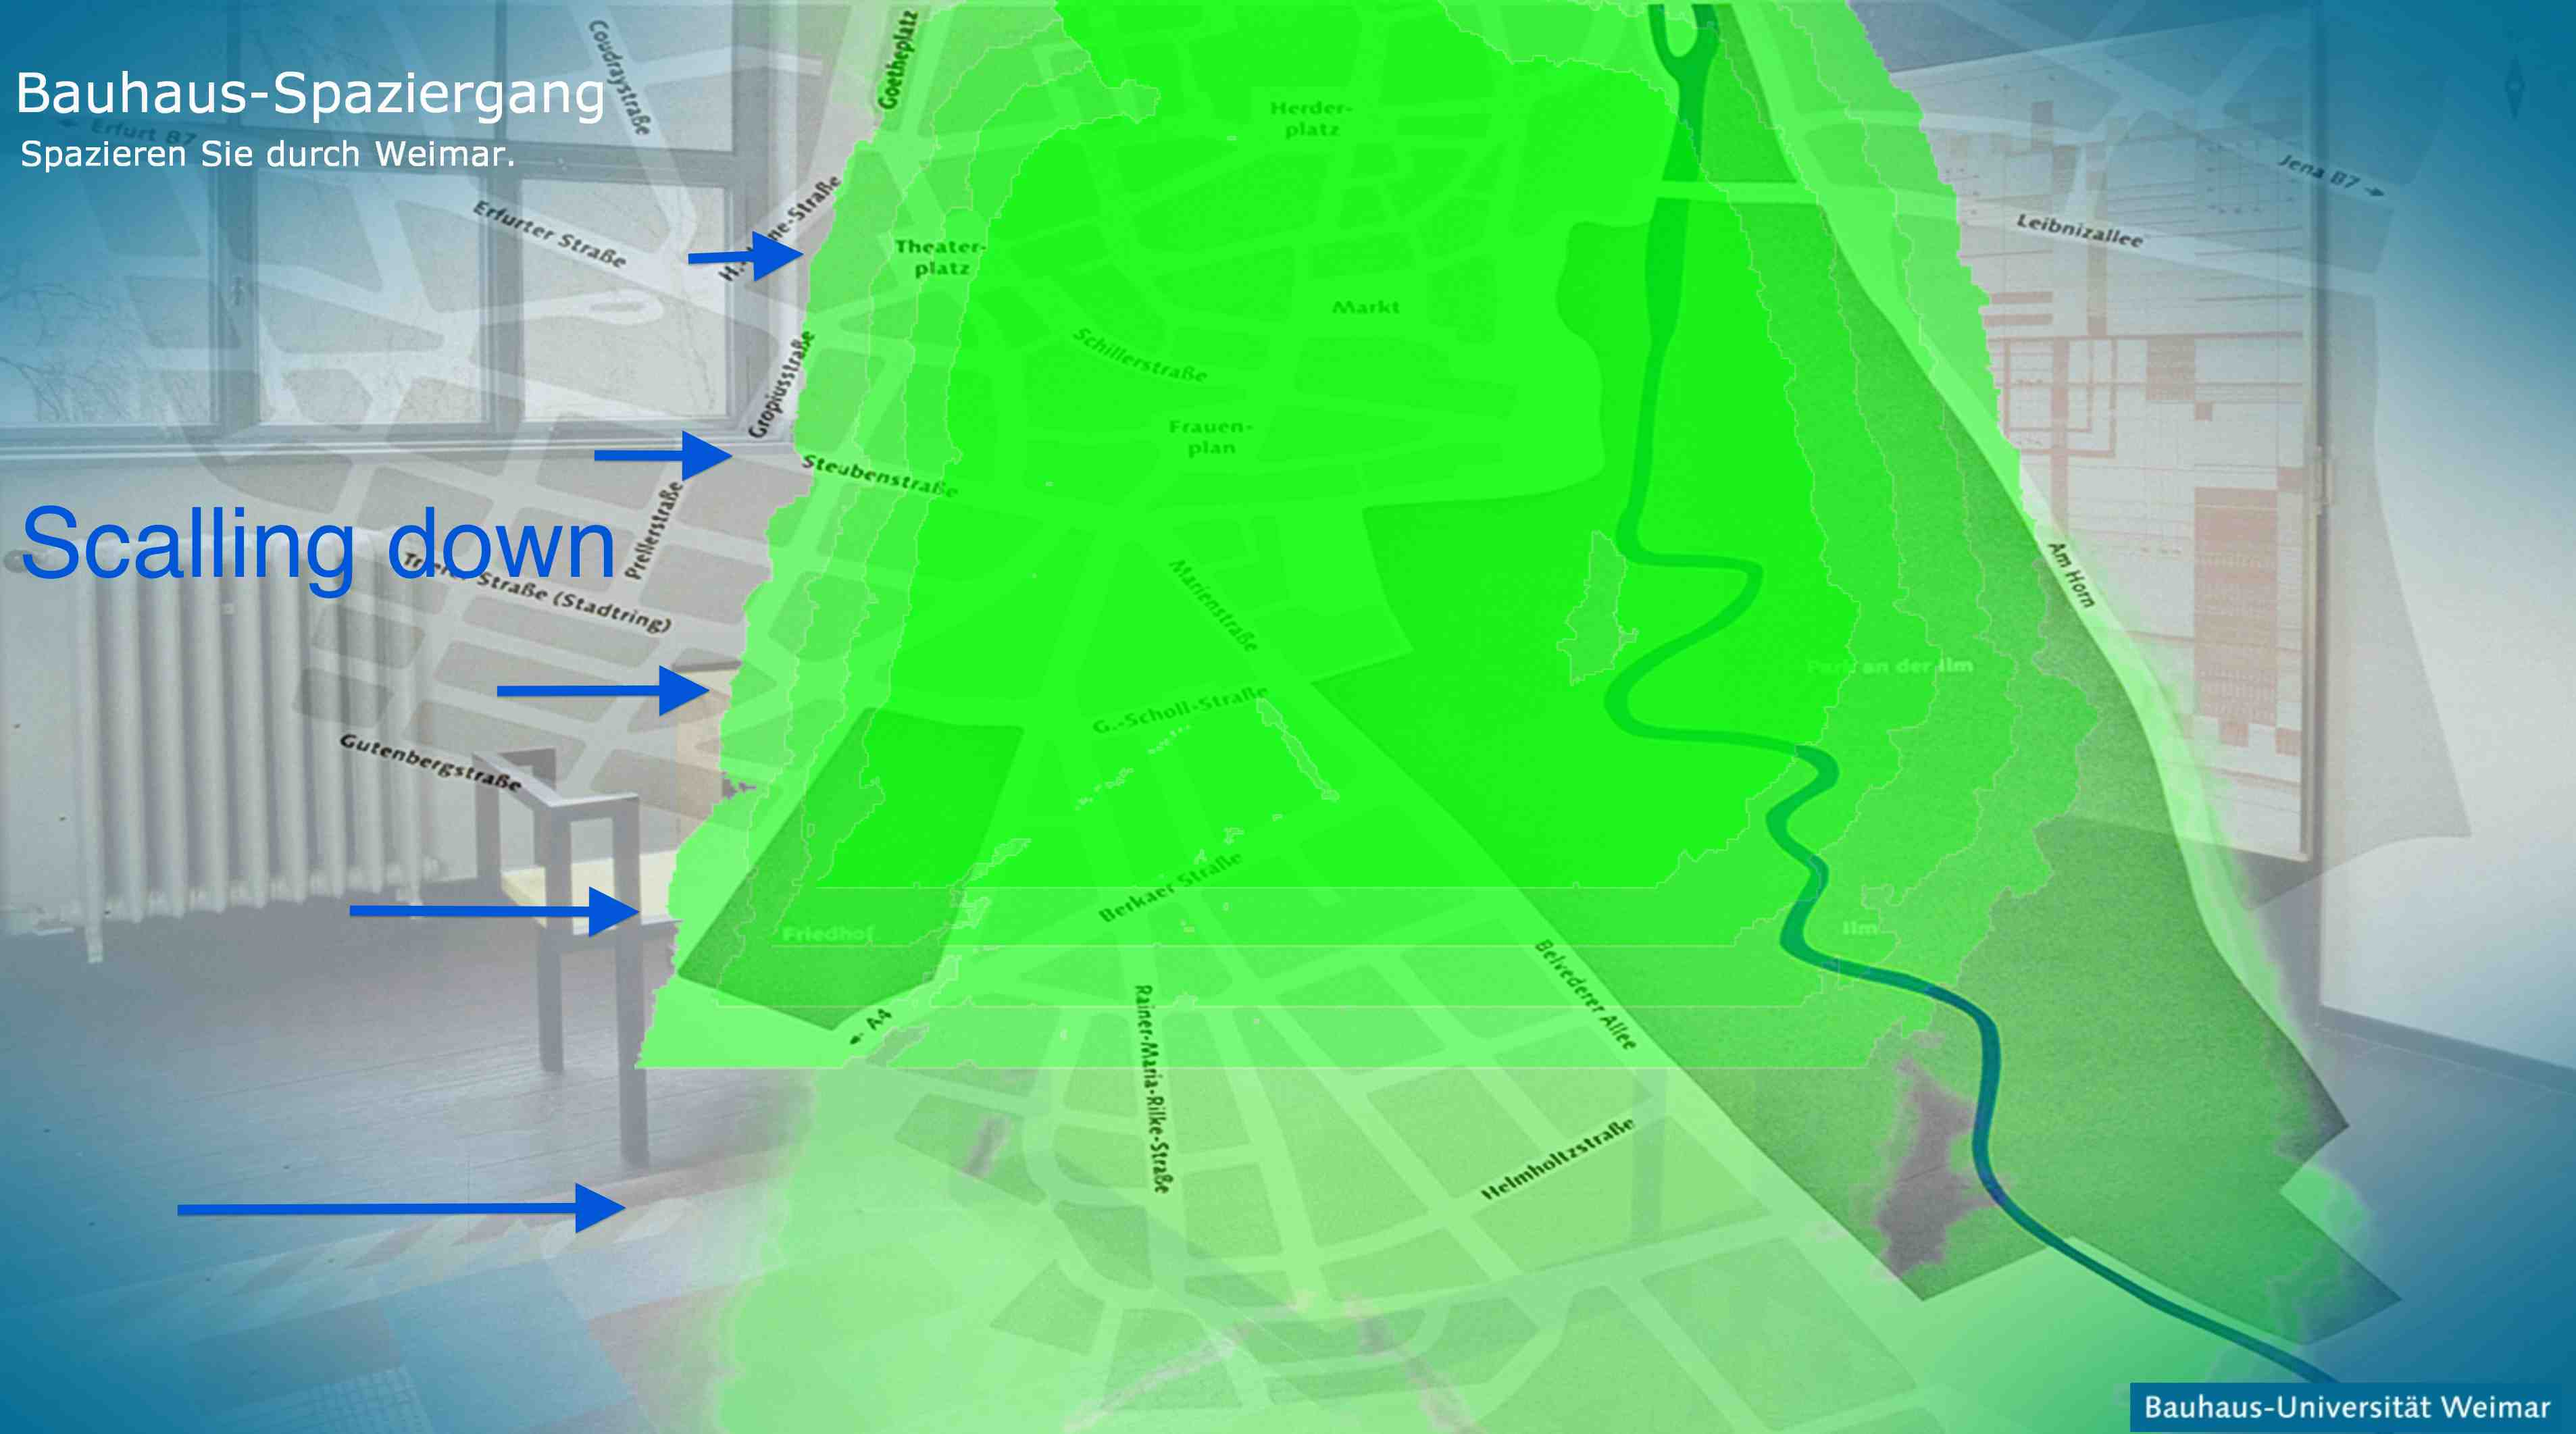
\includegraphics[width=40mm,height=30mm]{Figures/7/body_interactive/scalling_down} }}%
	\subfloat[]{{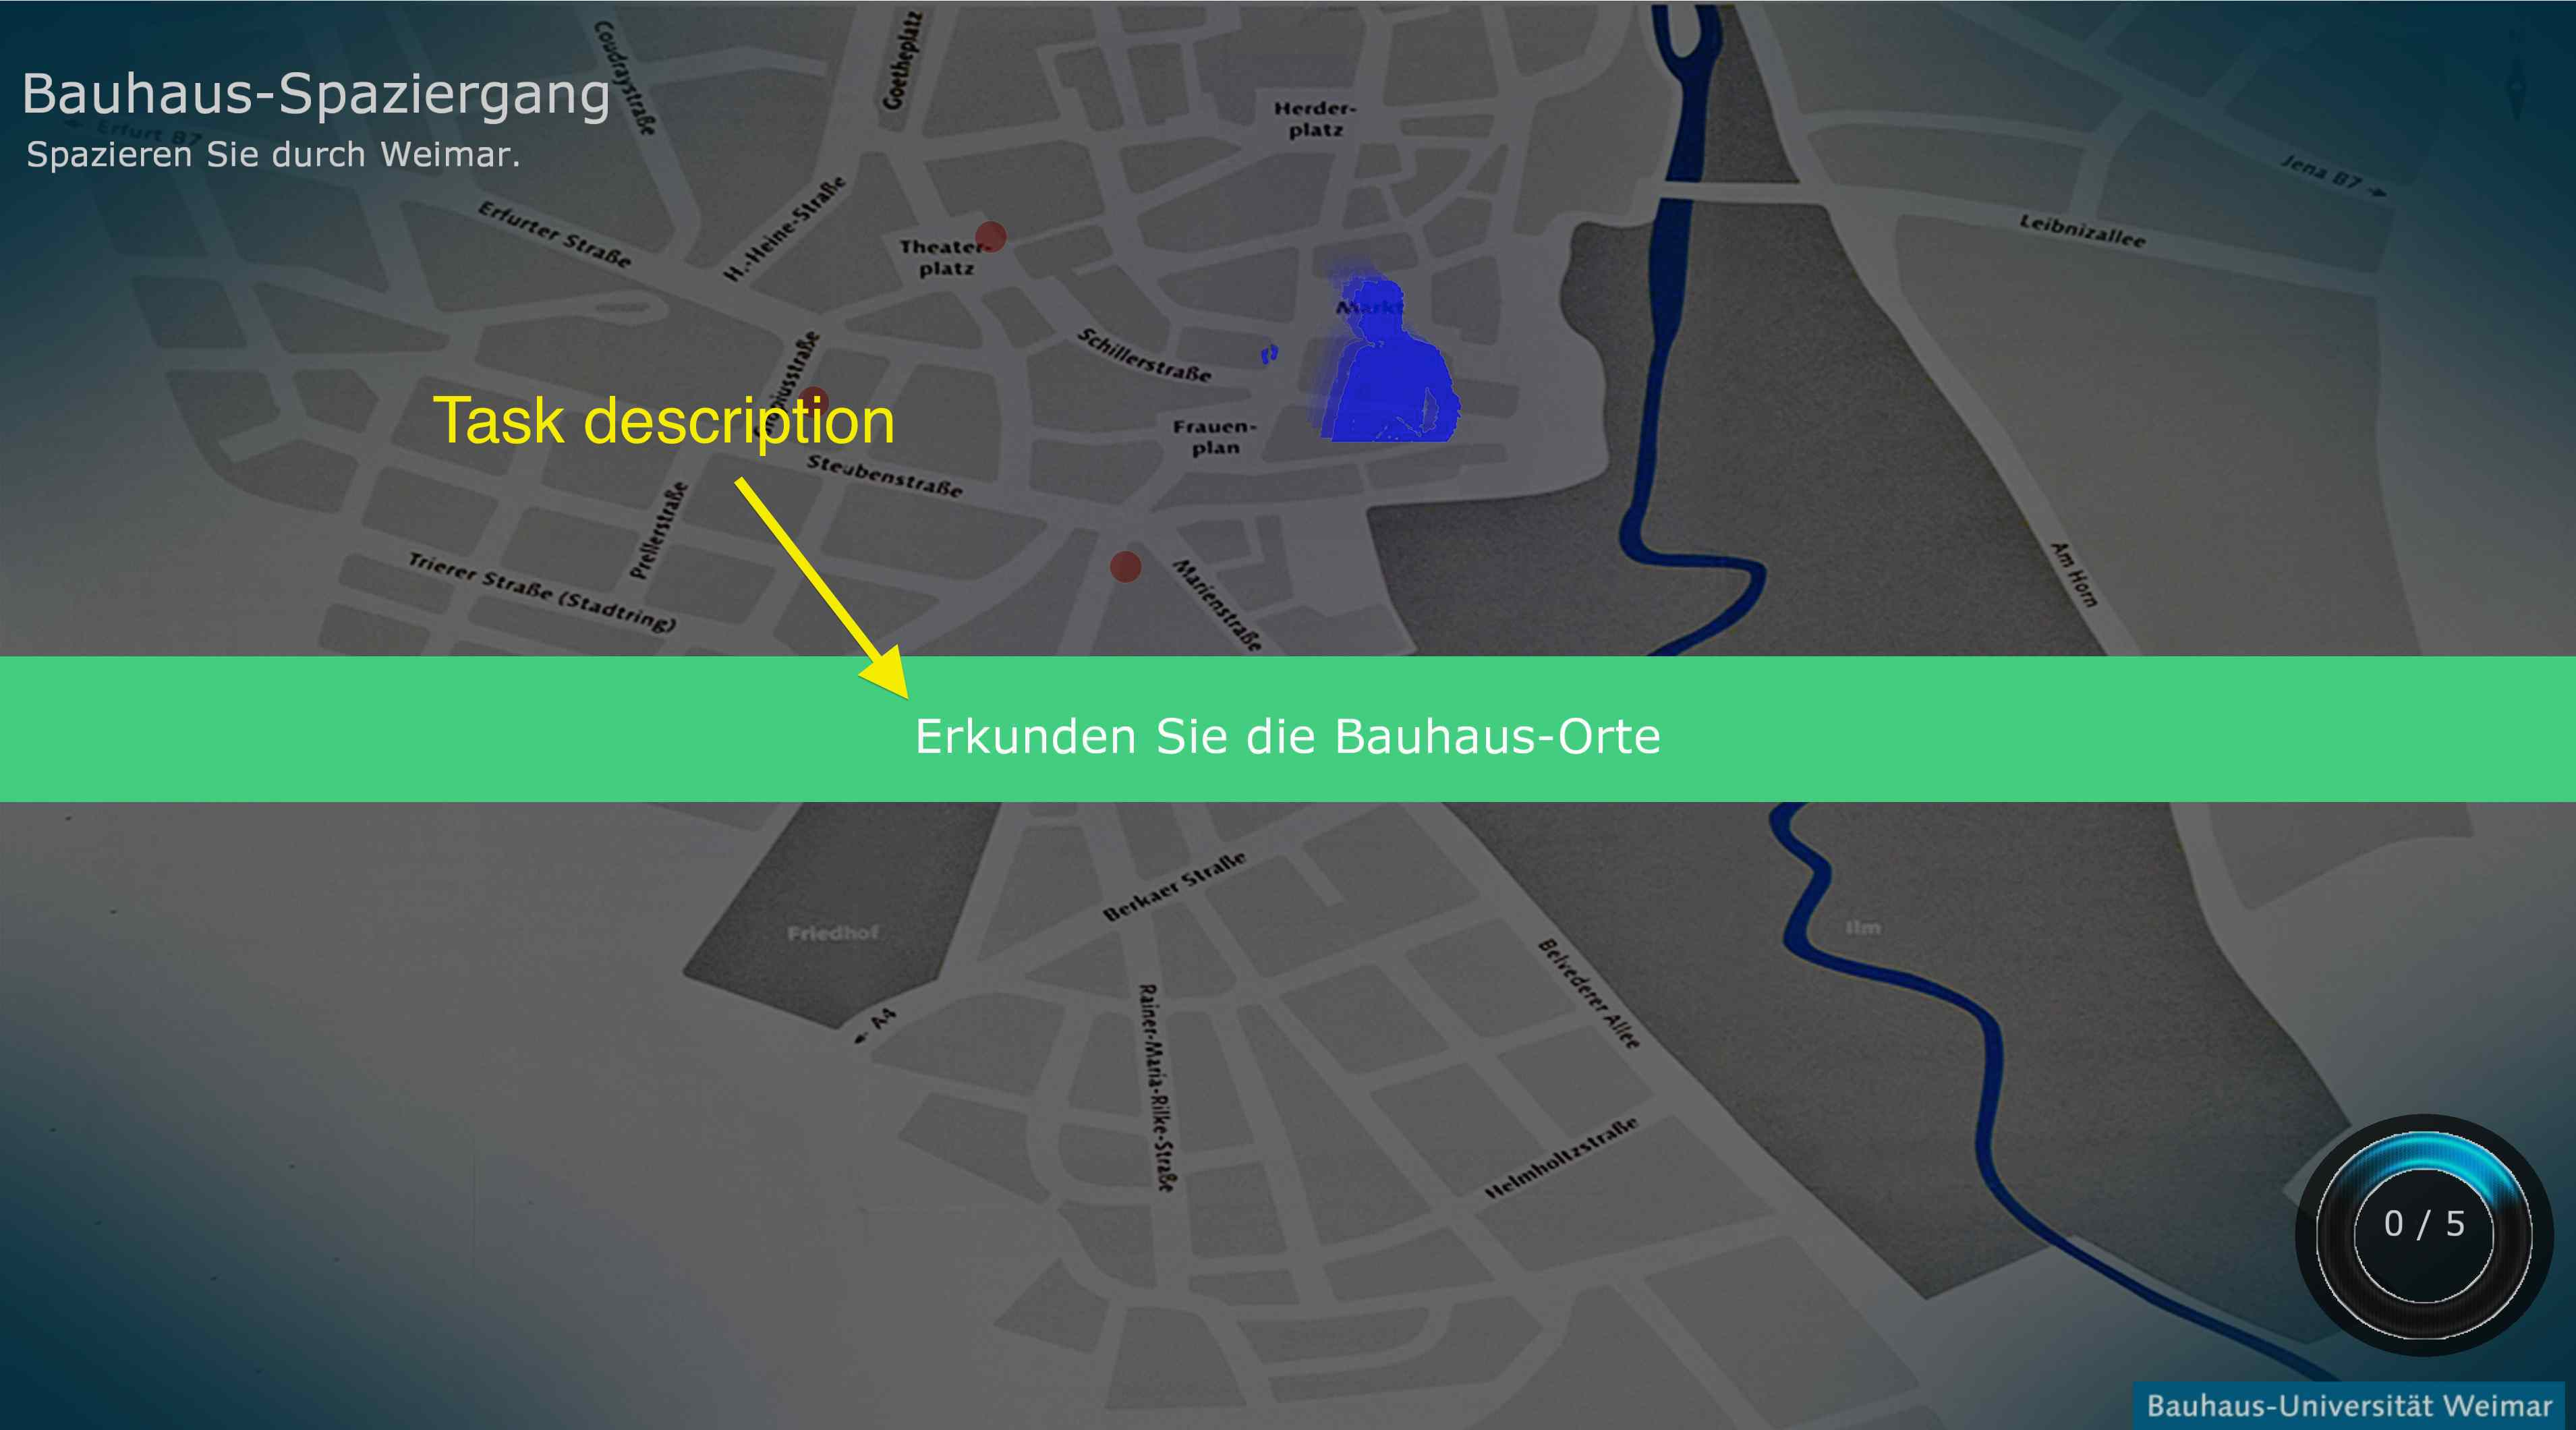
\includegraphics[width=40mm,height=30mm]{Figures/7/body_interactive/task_description} }}%
    \caption{As can be seen in picture A, the person is close to the screen and the loading animation is started, in picture B the person silhouette is being scaled down (in this example the silhouette color is green) and in picture C the instruction is shown. }%
    \label{fig:Switching_between_phases_body}%
\end{figure}


\subsubsection{Second interface}
In this interface participant can interact with the elements on the map.In bellow picture, the silhouette has visited two locations therefor has 2/5 score, to finish the interaction he needs to visit all the location or the timer on the corner right will be over.
\begin{figure}[H]
    \centering
    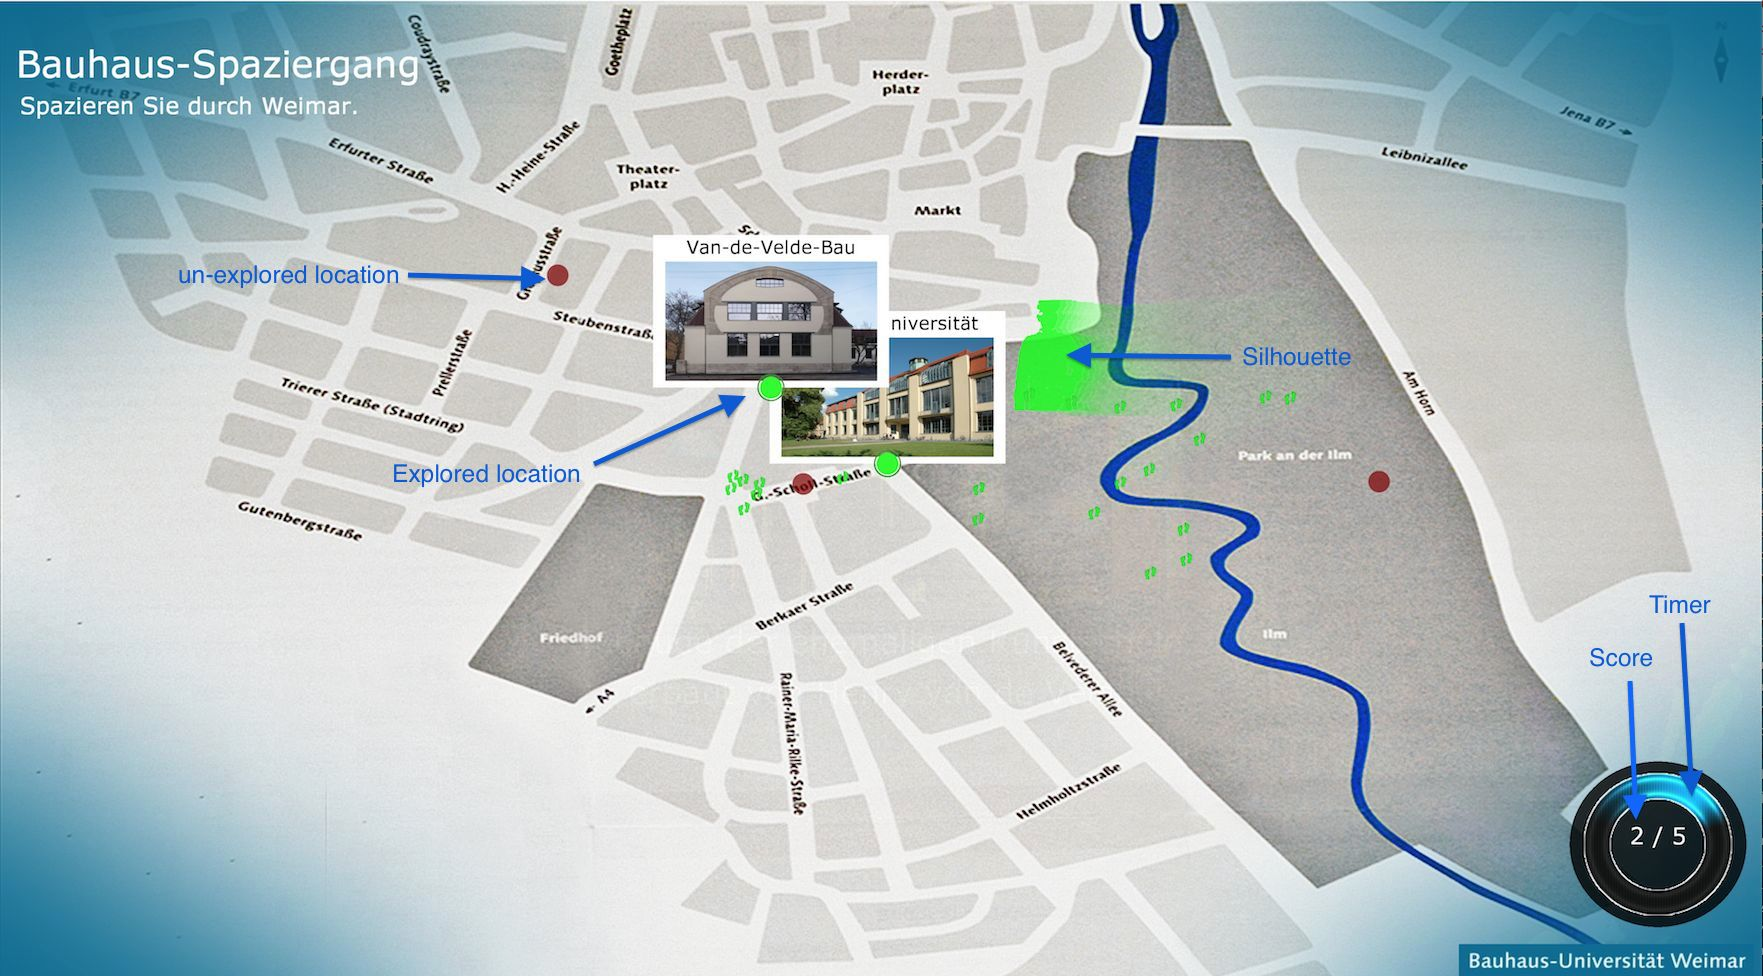
\includegraphics[width=100mm,height=60mm]{Figures/7/body_interactive/second_interface}
    \caption{Second Interface}%
    \label{fig:body_secondinterface}%
\end{figure}

\subsubsection{Flowchart Diagram}
The bellow chart roughly shows the flow of the application.
\begin{figure}[H]
    \centering
    \includegraphics[width=120mm,height=140mm]{Figures/7/body_interactive/body_flow_chart}
    \caption{Body Interactive advertisement Flowchart diagram}%
    \label{fig:Body_flowchat}%
\end{figure}


\subsubsection{Software Details}
The application is developed in Processing language with the support of Kinect Library, The application can run in Windows and OSX operating systems the system should have bellow requirements.

\begin{itemize}
\item Processing v2.2.2.
\item SimpleOpenNI library for Processing \cite{simpleopenni}
\item 32bit JRE (Java Runtime Environment) v1.8 or higher.
\item Windows / Mac OSX
\item RAM: 4GB or above.
\item CPU: Core i5 / i7 2.3Ghz
\end{itemize}

Refere to source code in DVD that has all the libraries and important things you require to run the application.


\subsection{Mobile Interactive application}
The interaction in this application is carried out with a smartphone, the interface is absolutely the same as the other two applications; the only different is that there is a colored circle pointer to select map elements.


\subsubsection{First screen interface}
This interface is designed in such a way to attract passers-by and also guide the participant on how to use their smartphone to access the advertisement application. The attraction is again the same method that was used for body, the passers-by silhouette is projected at the back of Access information. The interface has QR code that could be easy to be scanned instead of typing the whole IP address, and there is an alert area, that gets activated when a logged in person has not turned their phone in landscape orientation.

\begin{figure}[H]
    \centering
    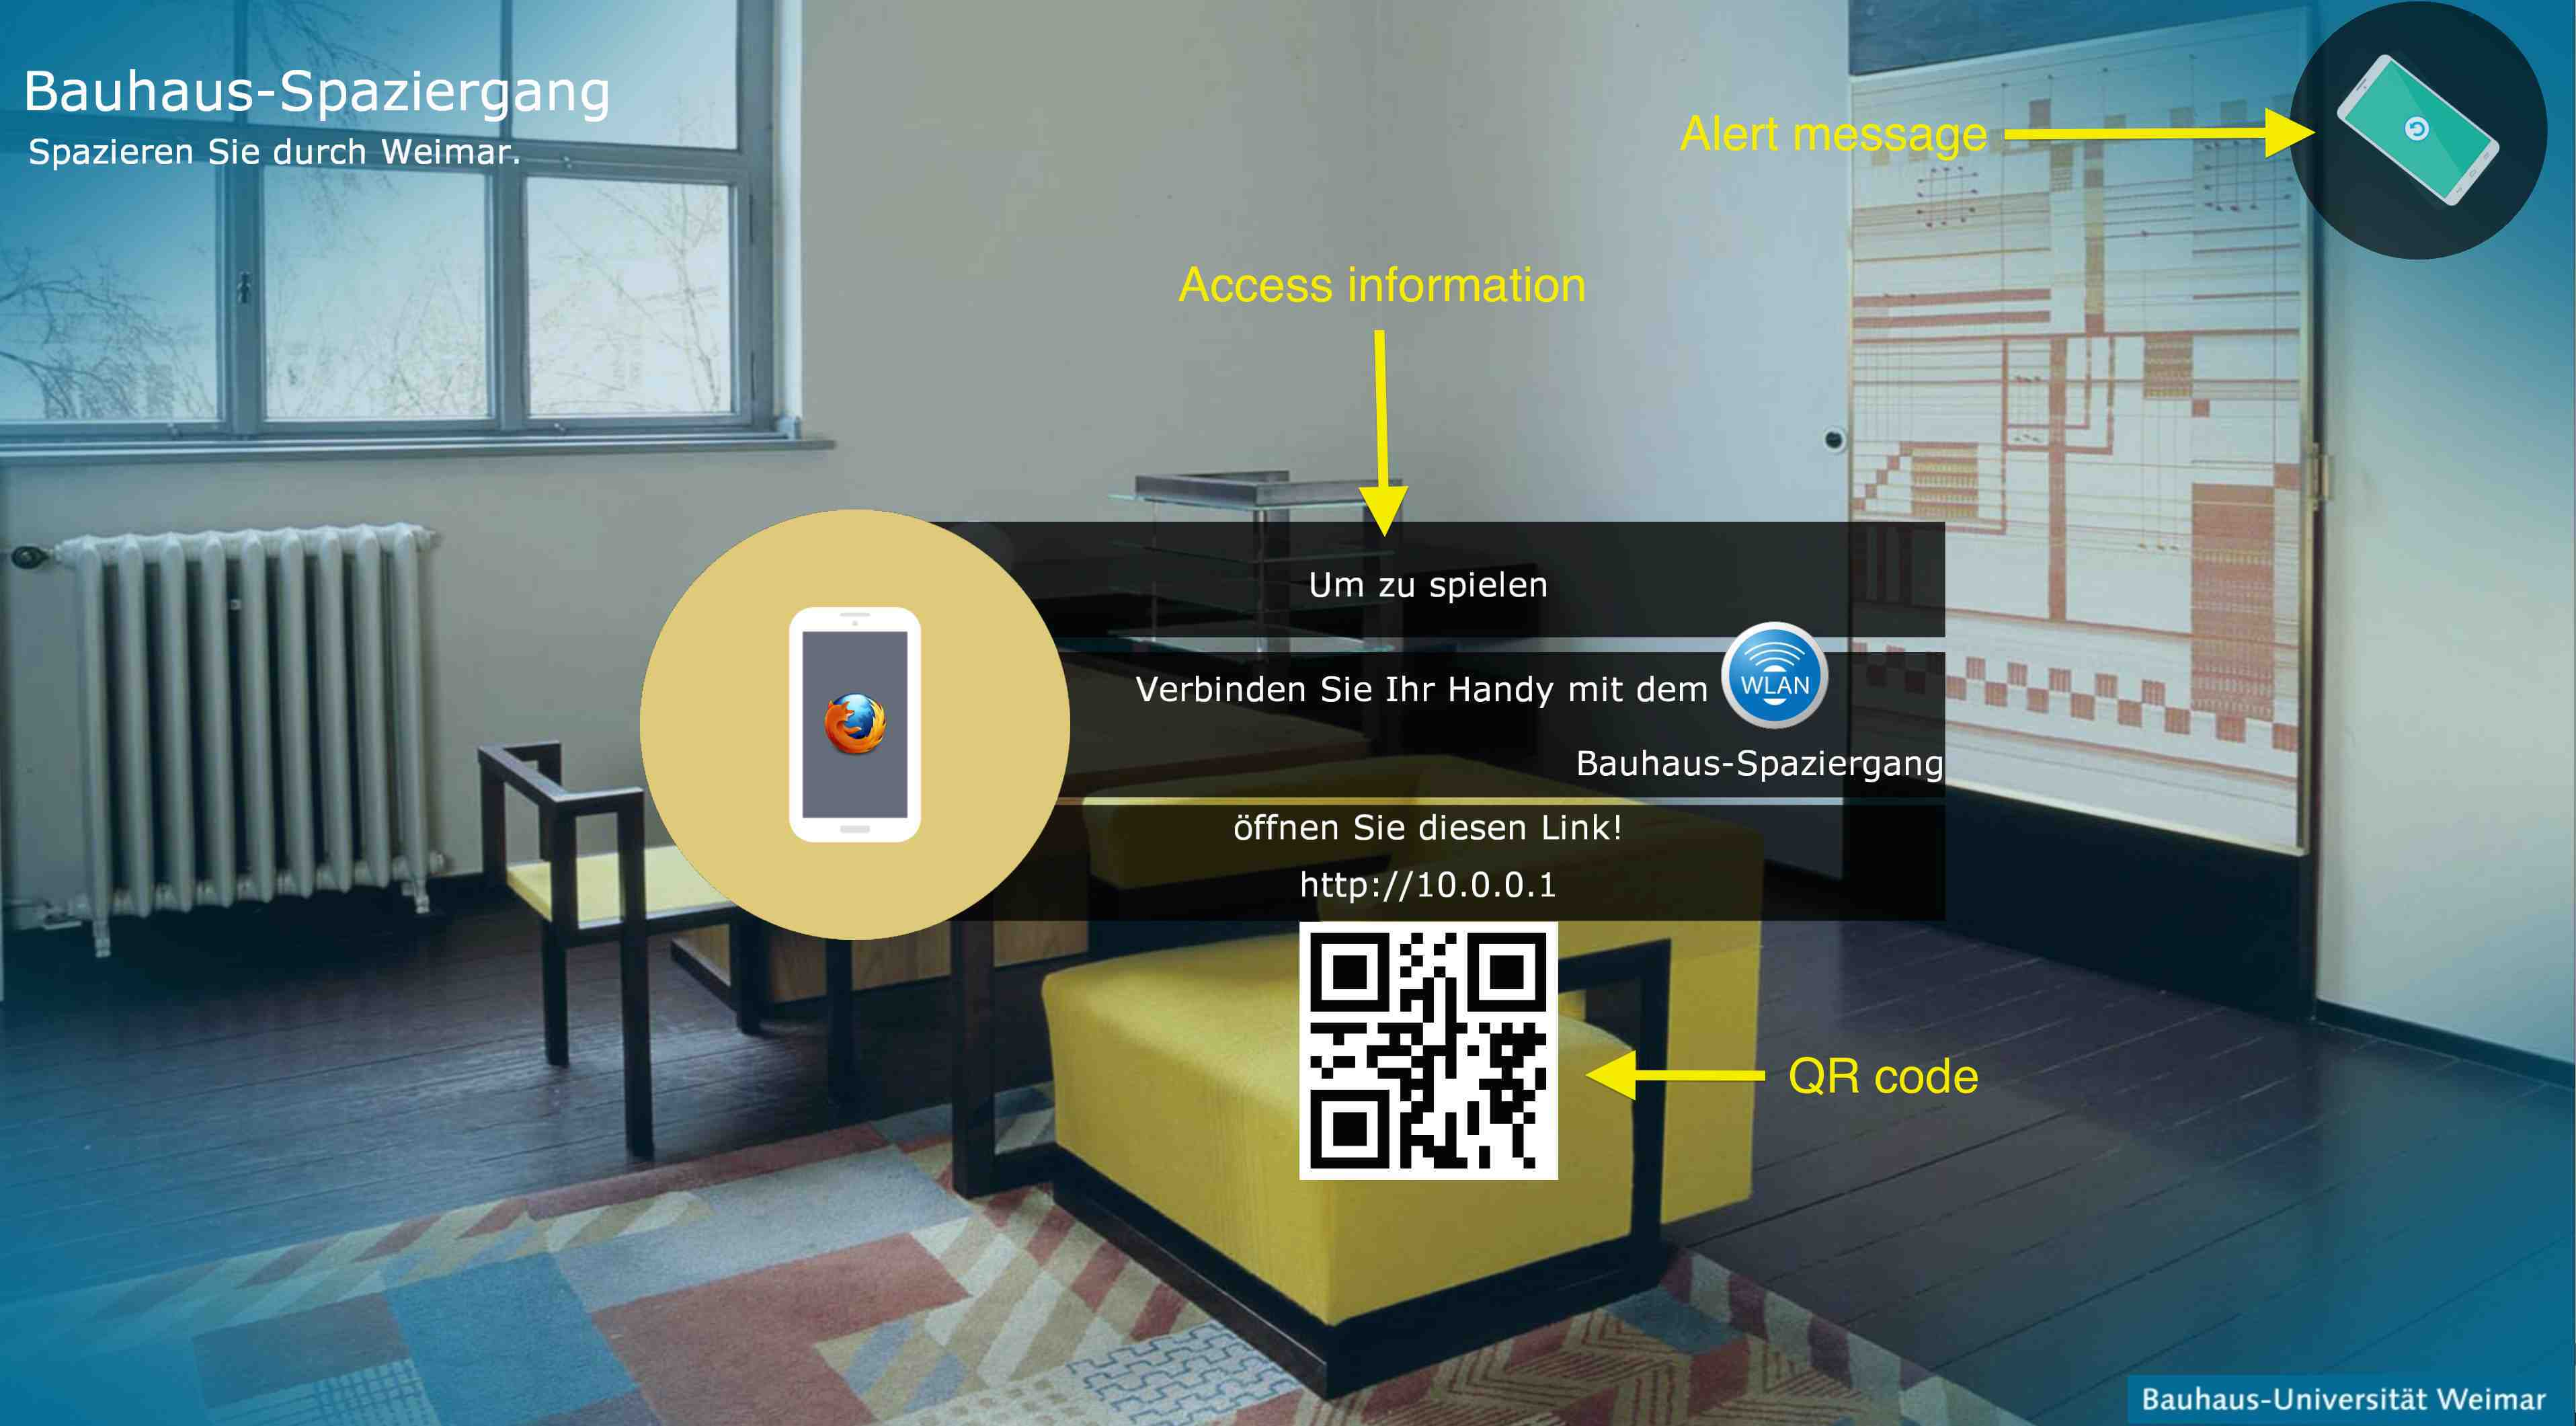
\includegraphics[width=100mm,height=60mm]{Figures/7/mobile_interactive/first_interface}
    \caption{Mobile interactive interface:}%
    \label{fig:mobile_firstinterface}%
\end{figure}



\subsubsection{Transition to second interfaces}
The first user will not be able to trigger the game, until his/her has not physically hold the phone in landscape, when it is in landscape the bellow process will be triggered.

\begin{enumerate}
\item Loading animation:\\
  The loading animation is a reaction to the action of the participants, and at the same time participants waits for something to be loaded.
\item  Creating Colored cursor: \\
A colored circle will be created for the participant in the center of the screen; each participant would have different colors matching to their controller interface in their phone.
\item Show task instruction:  \\
The instruction is fairly very easy and it is simplified in one sentence to explore locations on the map by using their phone.

\end{enumerate}

\begin{figure}[!htb]
    \centering
    \subfloat[]{{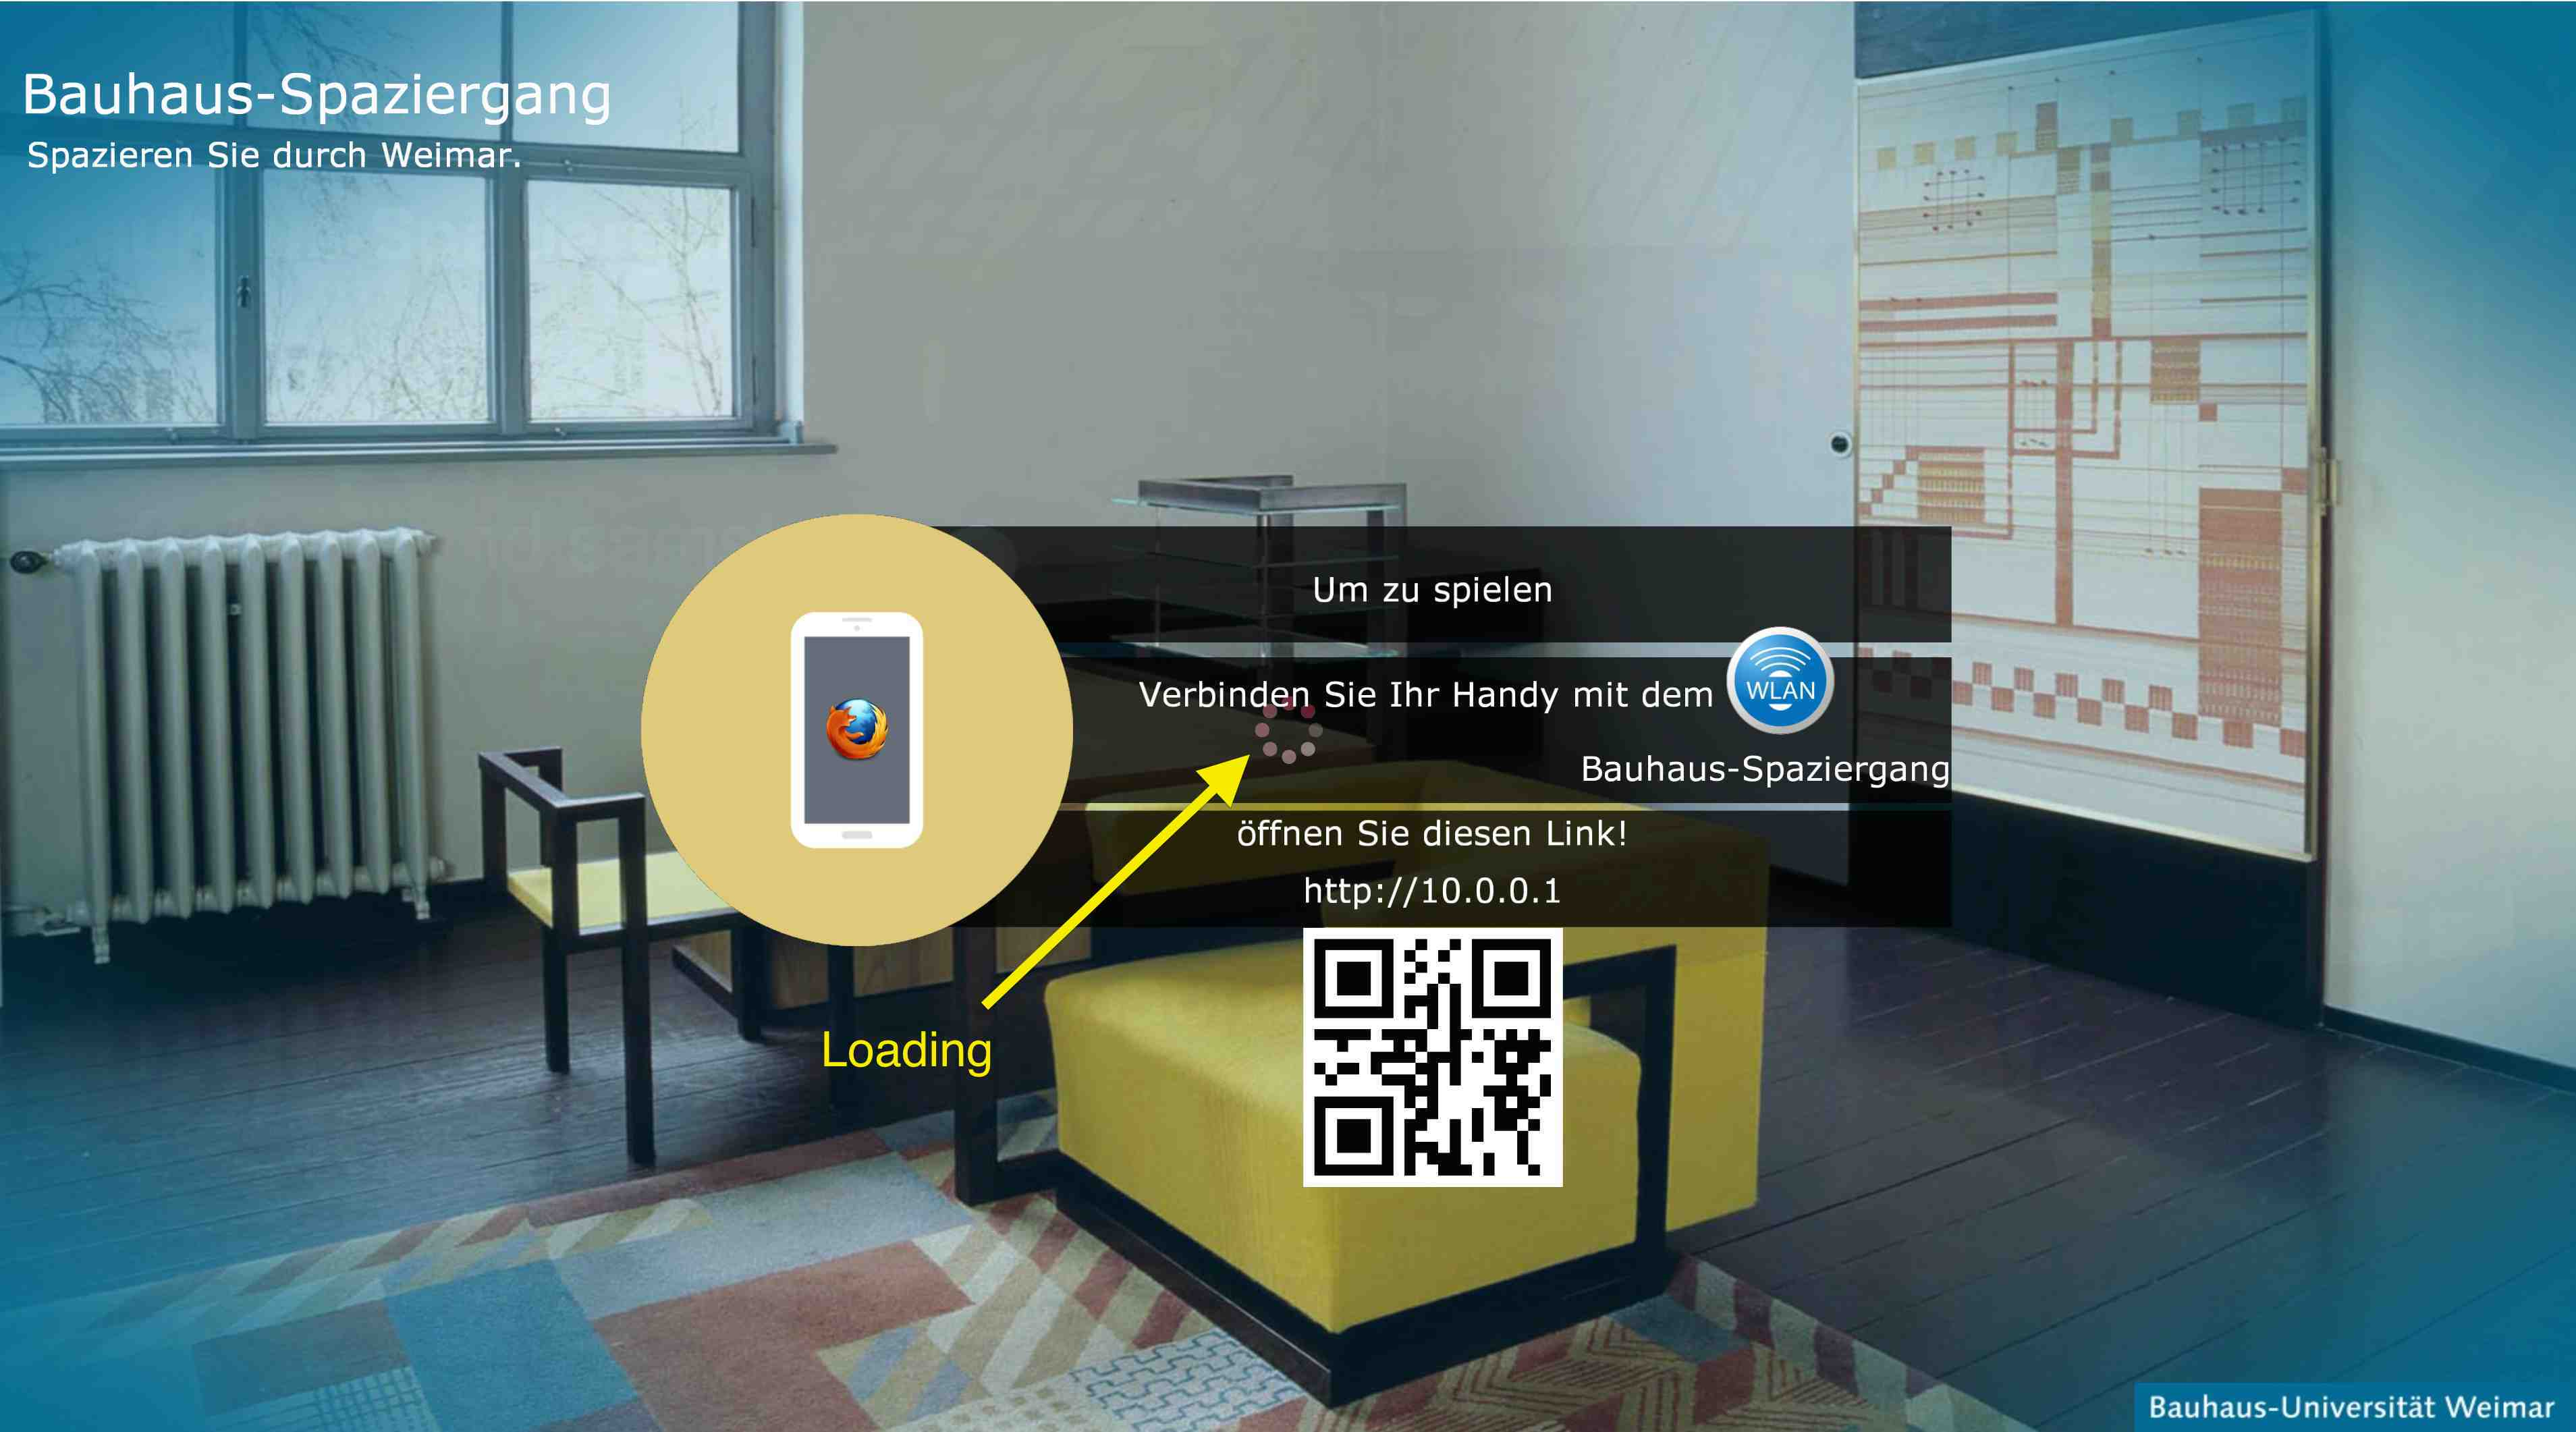
\includegraphics[width=50mm,height=40mm]{Figures/7/mobile_interactive/loading} }}%
	\subfloat[]{{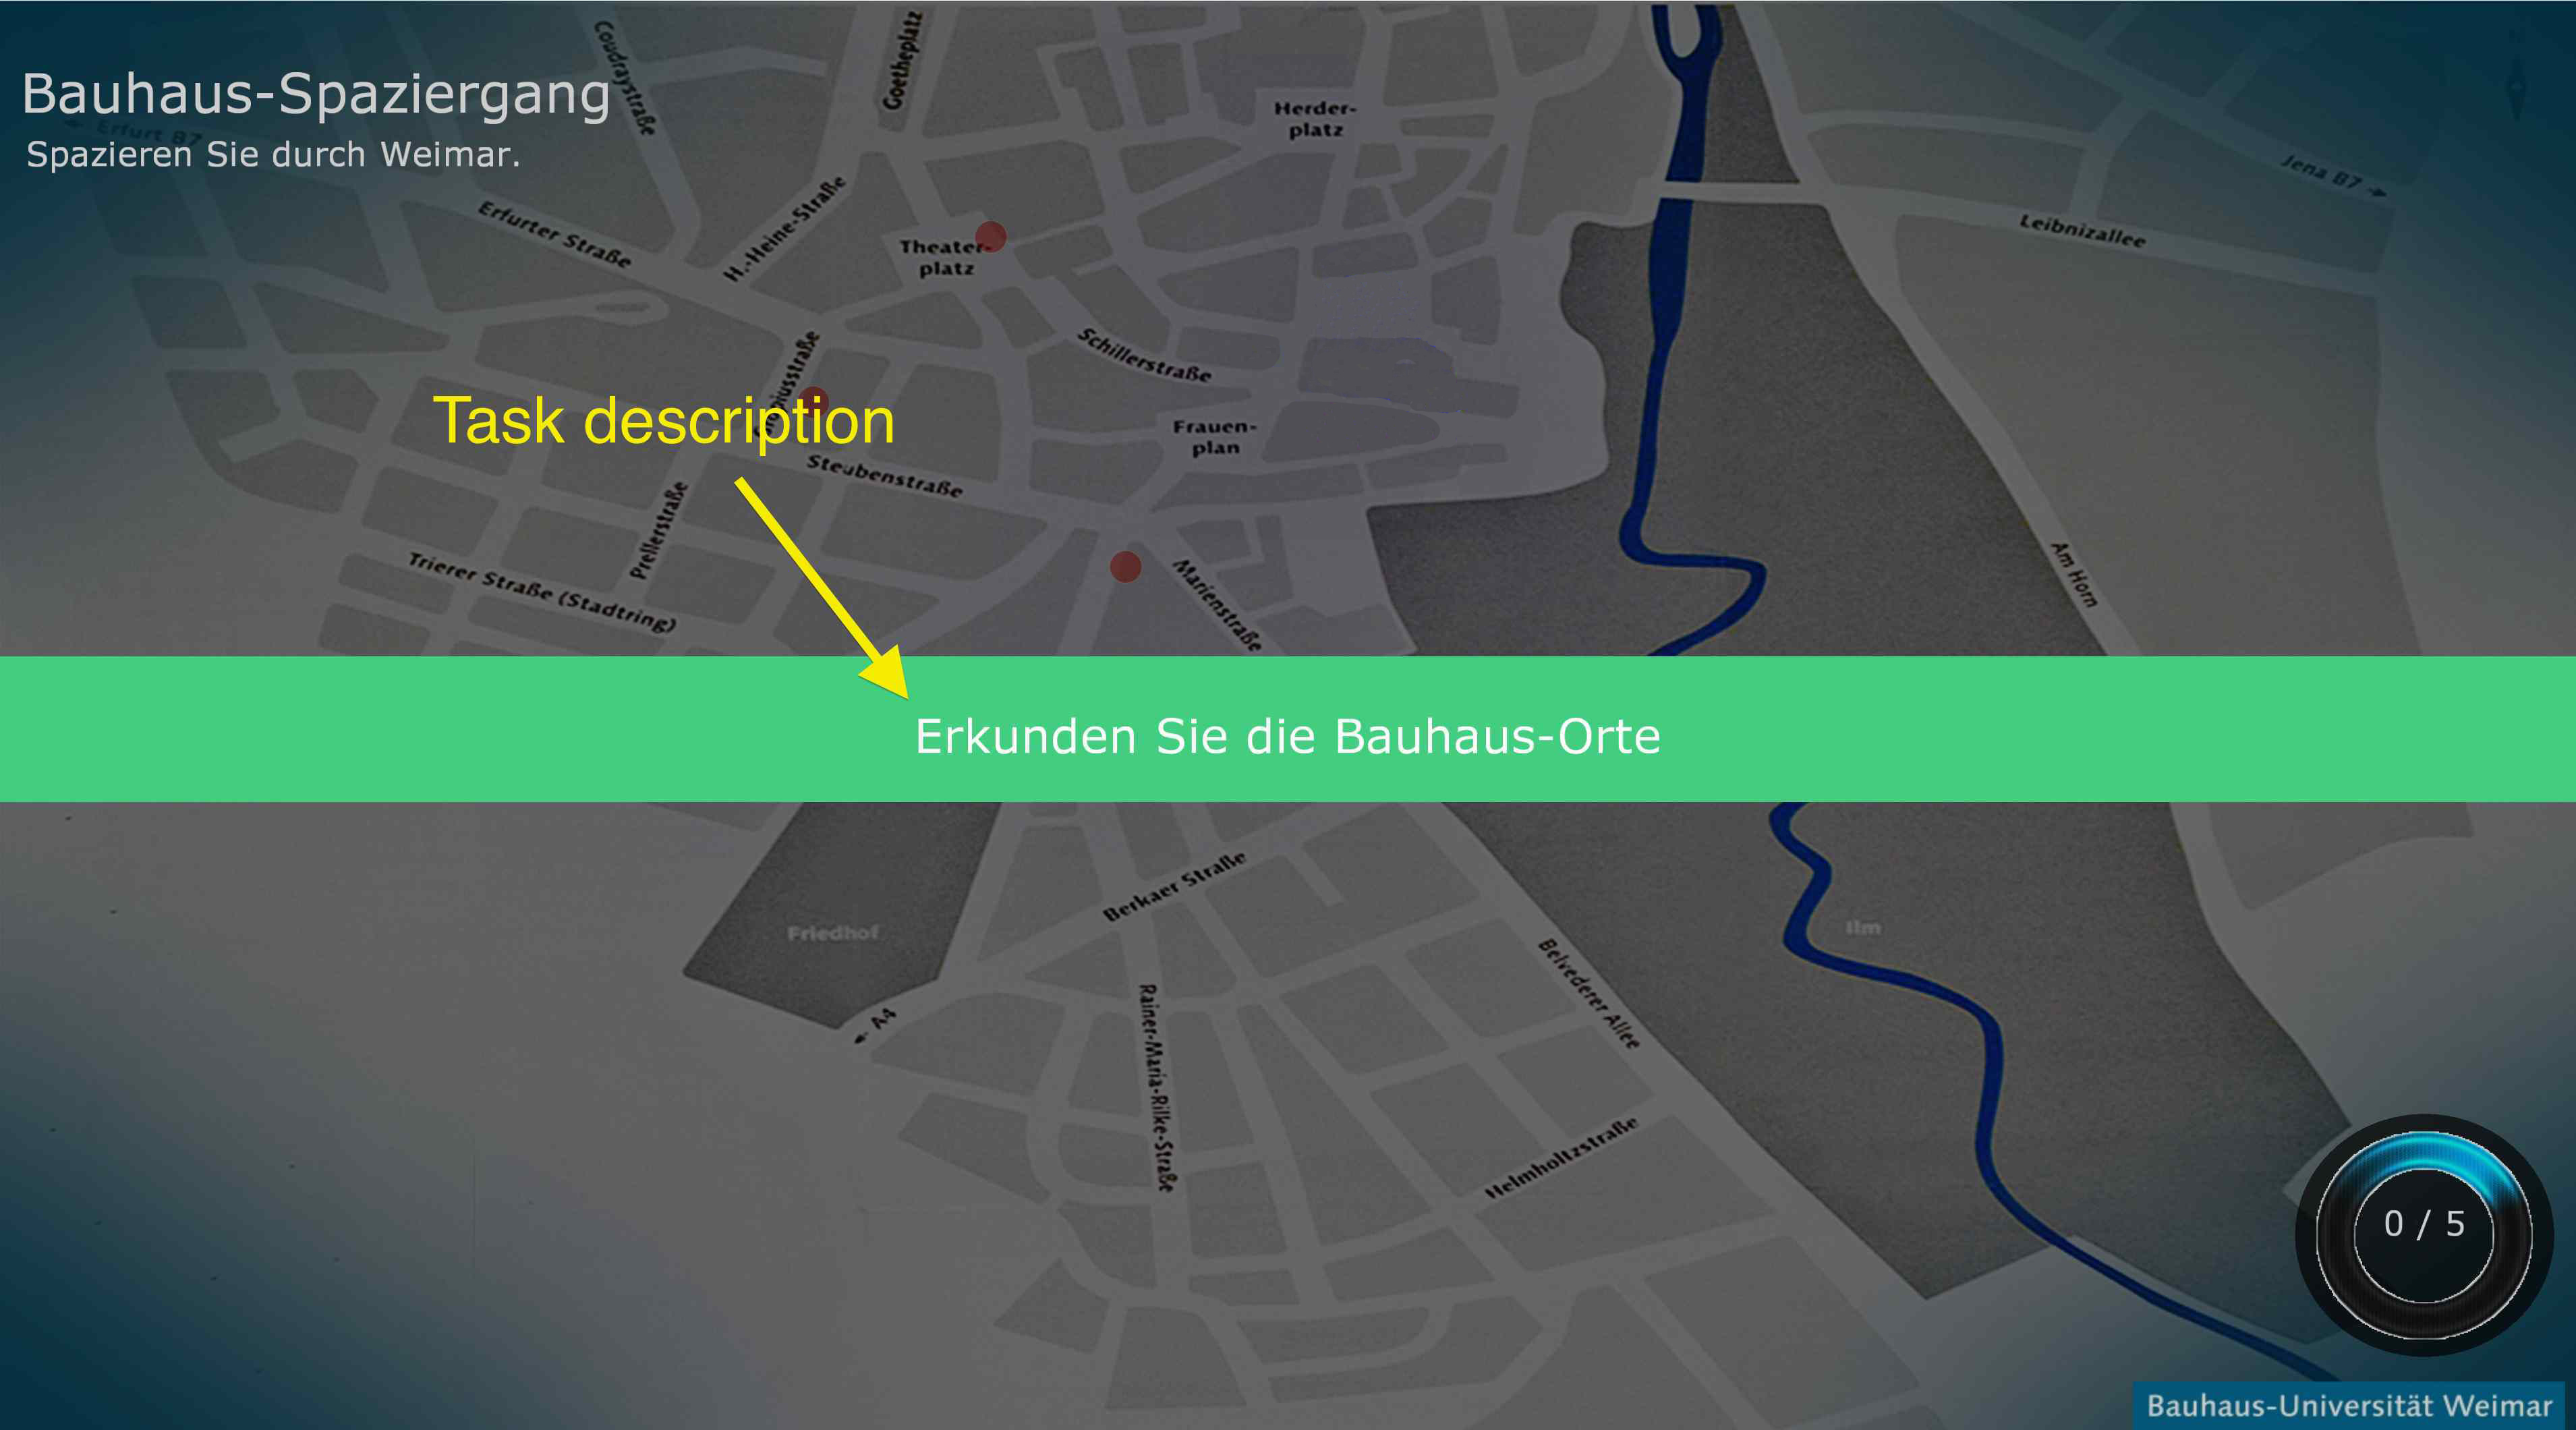
\includegraphics[width=50mm,height=40mm]{Figures/7/mobile_interactive/task_description} }}%
    \caption{In picture (A) a user has logged in and the screen is loading, in picture (B) the task description is shown.}%
    \label{fig:Switching_between_phases_mobile}%
\end{figure}



\subsubsection{Second screen interface}
Second screen is the interaction screen for the participants, participants can navigate the cursor using their phone controller page. As can be seen in bellow picture, the user is controlling the cursor and has explored one location, the user's defined name is also shown on the cursor, to provide a hint that they have reached an interest point a small circle is shown to determine the area of that interest point. The interaction will finishe when all the locations are explored or the interaction time finishes.


\begin{figure}[H]
    \centering
    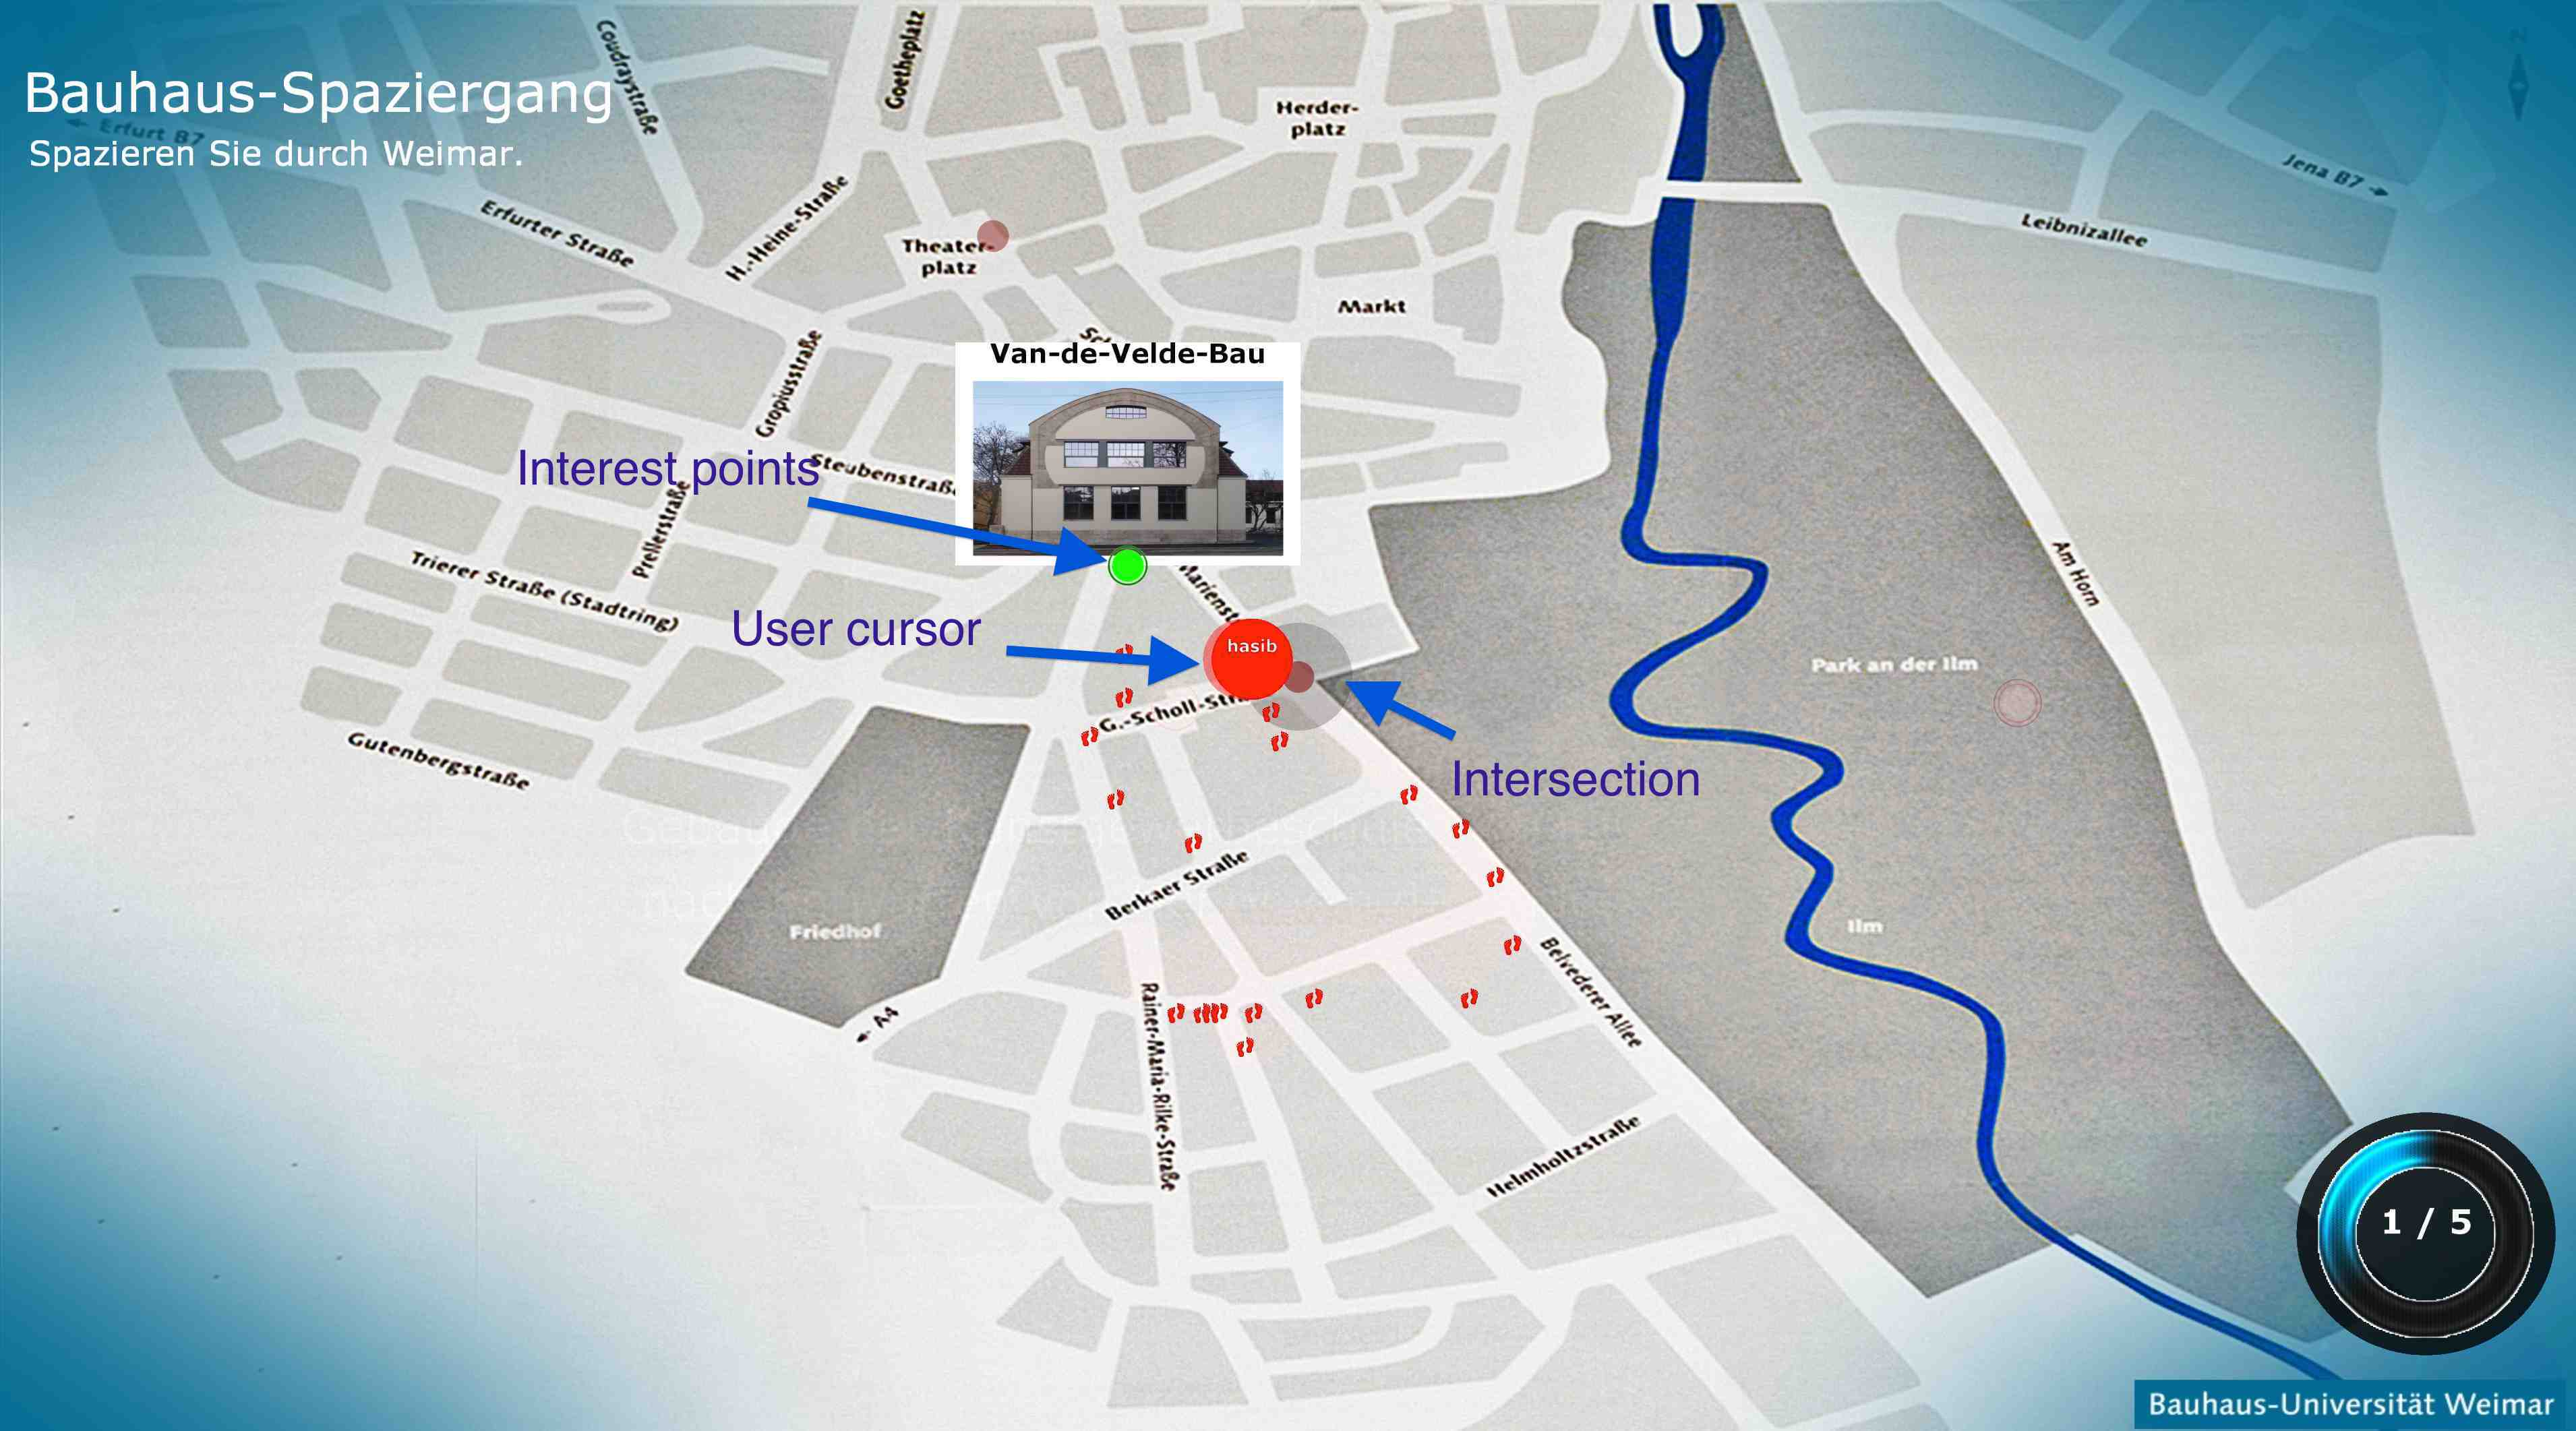
\includegraphics[width=100mm,height=60mm]{Figures/7/mobile_interactive/second_interface}
    \caption{Mobile interactive interface}%
    \label{fig:mobile_secondinterface}%
\end{figure}



\subsubsection{Mobile interface}
After opening the web page in smartphone, and entering name, the bellow interface would appear. The interface is very simply designed and has two elements, the cursor and the select button, with cursor the user can navigate inside the map for interest points and when reached on an interest point the participant presses the select button to explore that location, see the picture bellow.

\begin{figure}[H]
    \centering
    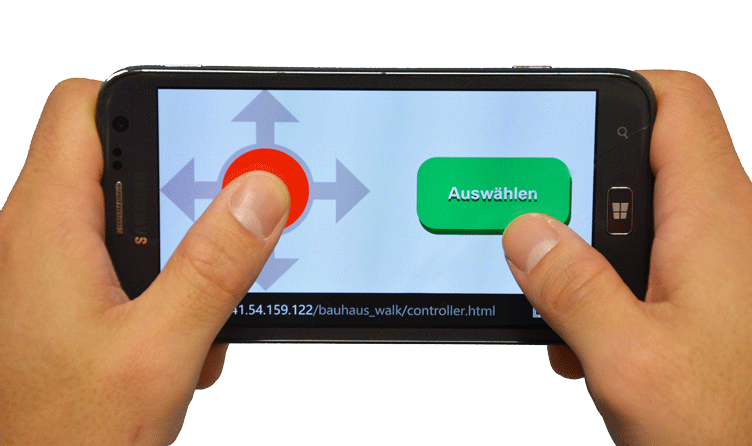
\includegraphics[width=100mm,height=60mm]{Figures/7/mobile_interactive/mobile_interface}
    \caption{Mobile controller interface: The left side is the cursor and the right side is the select button.}%
    \label{fig:mobile_controllerinterface}%
\end{figure}



\subsubsection{Hardware setup}
The hardware required for the type of interactive application, would be to use one Access point that enable participants to connect to the system, Kinect camera to record colored user images, a mobile phone at client side and obviously the screen and a workstation.


\begin{figure}[H]
    \centering
    \includegraphics[width=100mm,height=60mm]{Figures/7/mobile_interactive/Mobile_hardware_setup}
    \caption{Hardware setup}%
    \label{fig:mobile_hardware_setup}%
\end{figure}


\subsubsection{Software setup}
In order to make the system running we would need the bellow things.
\hilight{The controller is taken from another project MMM ball}
\begin{itemize}
\item Apache webserver:\\
The web server could be running in the same application system side-by-side. The web controller is using WebSocket client at the backend. Check the JavaScript configuration
file to have the IP address configured where application system is using.
\item Processing and WebSocket:\\
The application should be started and along that the WebSocket server should also be running silmultaniously. Processing should have WebSocket library installed before hand. The system should have a valid IP address to be reached by webserver.
\item OpenProcessing Library:\\
Processing should have OpenProcessing library installed to be able to run Kinect Camera for color image recording.
\end{itemize}


\begin{figure}[H]
    \centering
    \includegraphics[width=120mm,height=60mm]{Figures/7/mobile_interactive/mobile_software}
    \caption{System architecture}%
    \label{fig:mobile_software_setup}%
\end{figure}

To have a full look to the software, please refer to the DVD to see all the source codes and the relavent applications.

\subsubsection{Flowchart Diagram}
The bellow chart roughly shows the flow of the application.
\begin{figure}[H]
    \centering
    \includegraphics[width=130mm,height=160mm]{Figures/7/mobile_interactive/mobile_flow_chart}
    \caption{Mobile Interactive advertisement Flowchart diagram}%
    \label{fig:mobile_flowchat}%
\end{figure}



